\subsection{Nestor example 3}
%

% - Purpose & Problem description:
%     These first two parts give reader short details about the test case,
%     the physical phenomena involved and specify how the numerical solution will be validated
%
\subsubsection{Purpose}
%
Third test example for Nestor
%
\subsubsection{Description of the problem}
%
This example performs the maintenace of a fairway. The dredged material will be transfered (dumped) in the dumping area.


The fairway and the dumping area (see Figure \ref{grid}) are defined by polygons which are defined in file \texttt{\_DigPolys.dat}.



Convention for naming polygons: The polygon name must start with an integer between 100 and 999. Any text after that is treated as a comment to  help the user. 
Internally only the number is used to identify the polygon. 


% - Reference:
%     This part gives the reference solution we are comparing to and
%     explicits the analytical solution when available;
%
%
\subsubsection{Reference}
%

% - Physical parameters:
%     This part specifies the geometry, details all the physical parameters
%     used to describe both porous media (soil model in particularly) and
%     solute characteristics (dispersion/diffusion coefficients, soil <=> pollutant interactions...)
%
%
\subsubsection{Physical parameters}
%
The simulation is set up with ten grain classes. 
The bottom is discretised with three layers. A constant active layer (0.1 m), an underlying stratum (0.1 m) and a third layer up to the rigid bed (9.8m).  

The Meyer-Peter Mueller (MPM) transport formula is used but the MPM parameter is set to 16 to create a bigger dynamic in the bottom elevation. Thus all bottom changes are a result of the sediment transport, digging and dumping processes.  
% - Geometry and Mesh:
%     This part describes the mesh used in the computation
%
%
\subsubsection{Geometry and Mesh}
%
A 3.3 km long flume with two 180 degree bends has been chosen as test geometry.
The width of the flume is 200 m  (see Figure \ref{grid}). 

The mesh consists of 1614 nodes and 2948 elements.

\begin{figure} [!h]
\centering
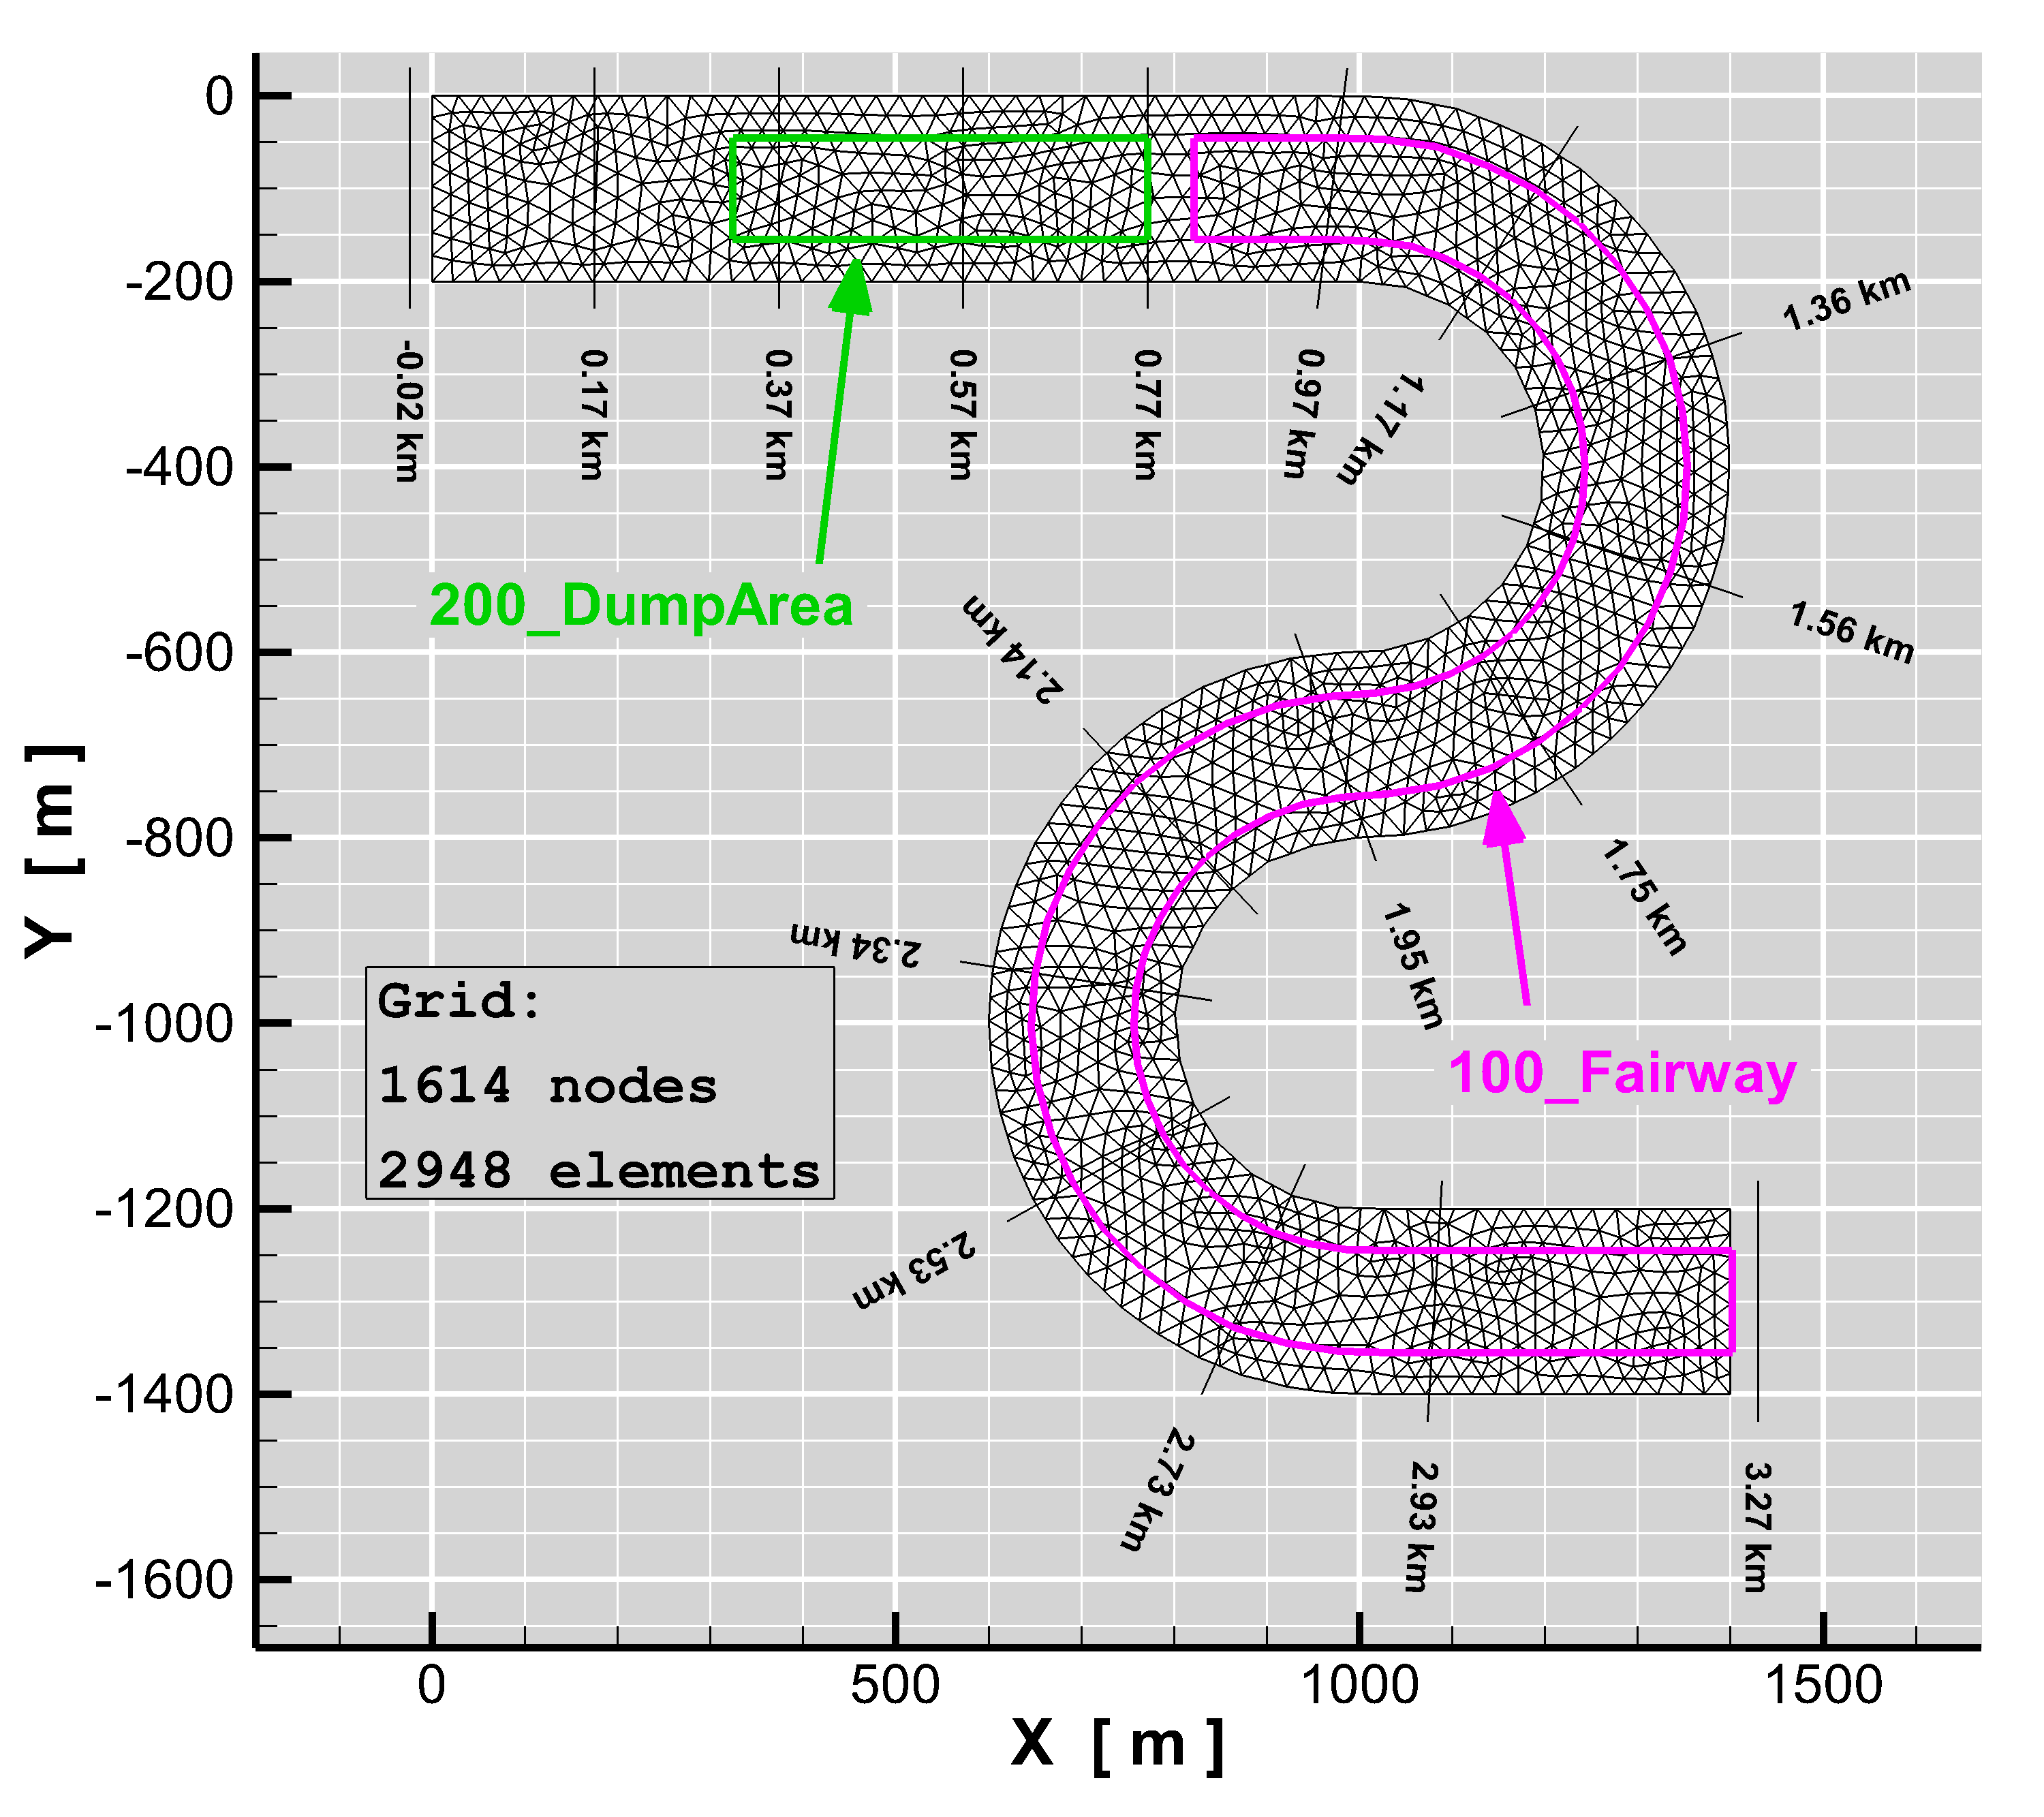
\includegraphics[scale=0.14]{../img/critDig_grid_Polys_2D.png}
\caption{Geometry of the test flume with two bends and the two polygons}\label{grid}
\end{figure}


% - Initial and boundary conditions:
%     This part details both initial and boundary conditions used to simulate the case
%
%
\subsubsection{Initial and Boundary Conditions}
%
Steady state boundary conditions:
\begin{itemize}
\item{ Discharge at the inlet = 1000 m$^3$/s}
\item Water level at outlet = 2.2 m
\item Sedimentological equilibrium at the inlet (zF is constant, QS will be calculated)
\end{itemize}
Fully developed flow and bottom from a previous simulation is used as initial conditions.

The total simulation period is 777600.0000 s (9 days)
with a time step of 6 s . 
% - Numerical parameters:
%     This part is used to specify the numerical parameters used
%     (adaptive time step, mass-lumping when necessary...)
%
%
\subsubsection{Numerical parameters}
%
% - Results:
%     We comment in this part the numerical results against the reference ones,
%     giving understanding keys and making assumptions when necessary.
%
%
\subsubsection{Results}
%
Figure \ref{result50} shows the evolution after 0s, 70s and 150s. The digging and dumping happens between 0 an 1 h and between 192 and 193 h .

% Here is an example of how to include the graph generated by validateTELEMAC.py
% They should be in test_case/img
\begin{figure} [!h]
\centering
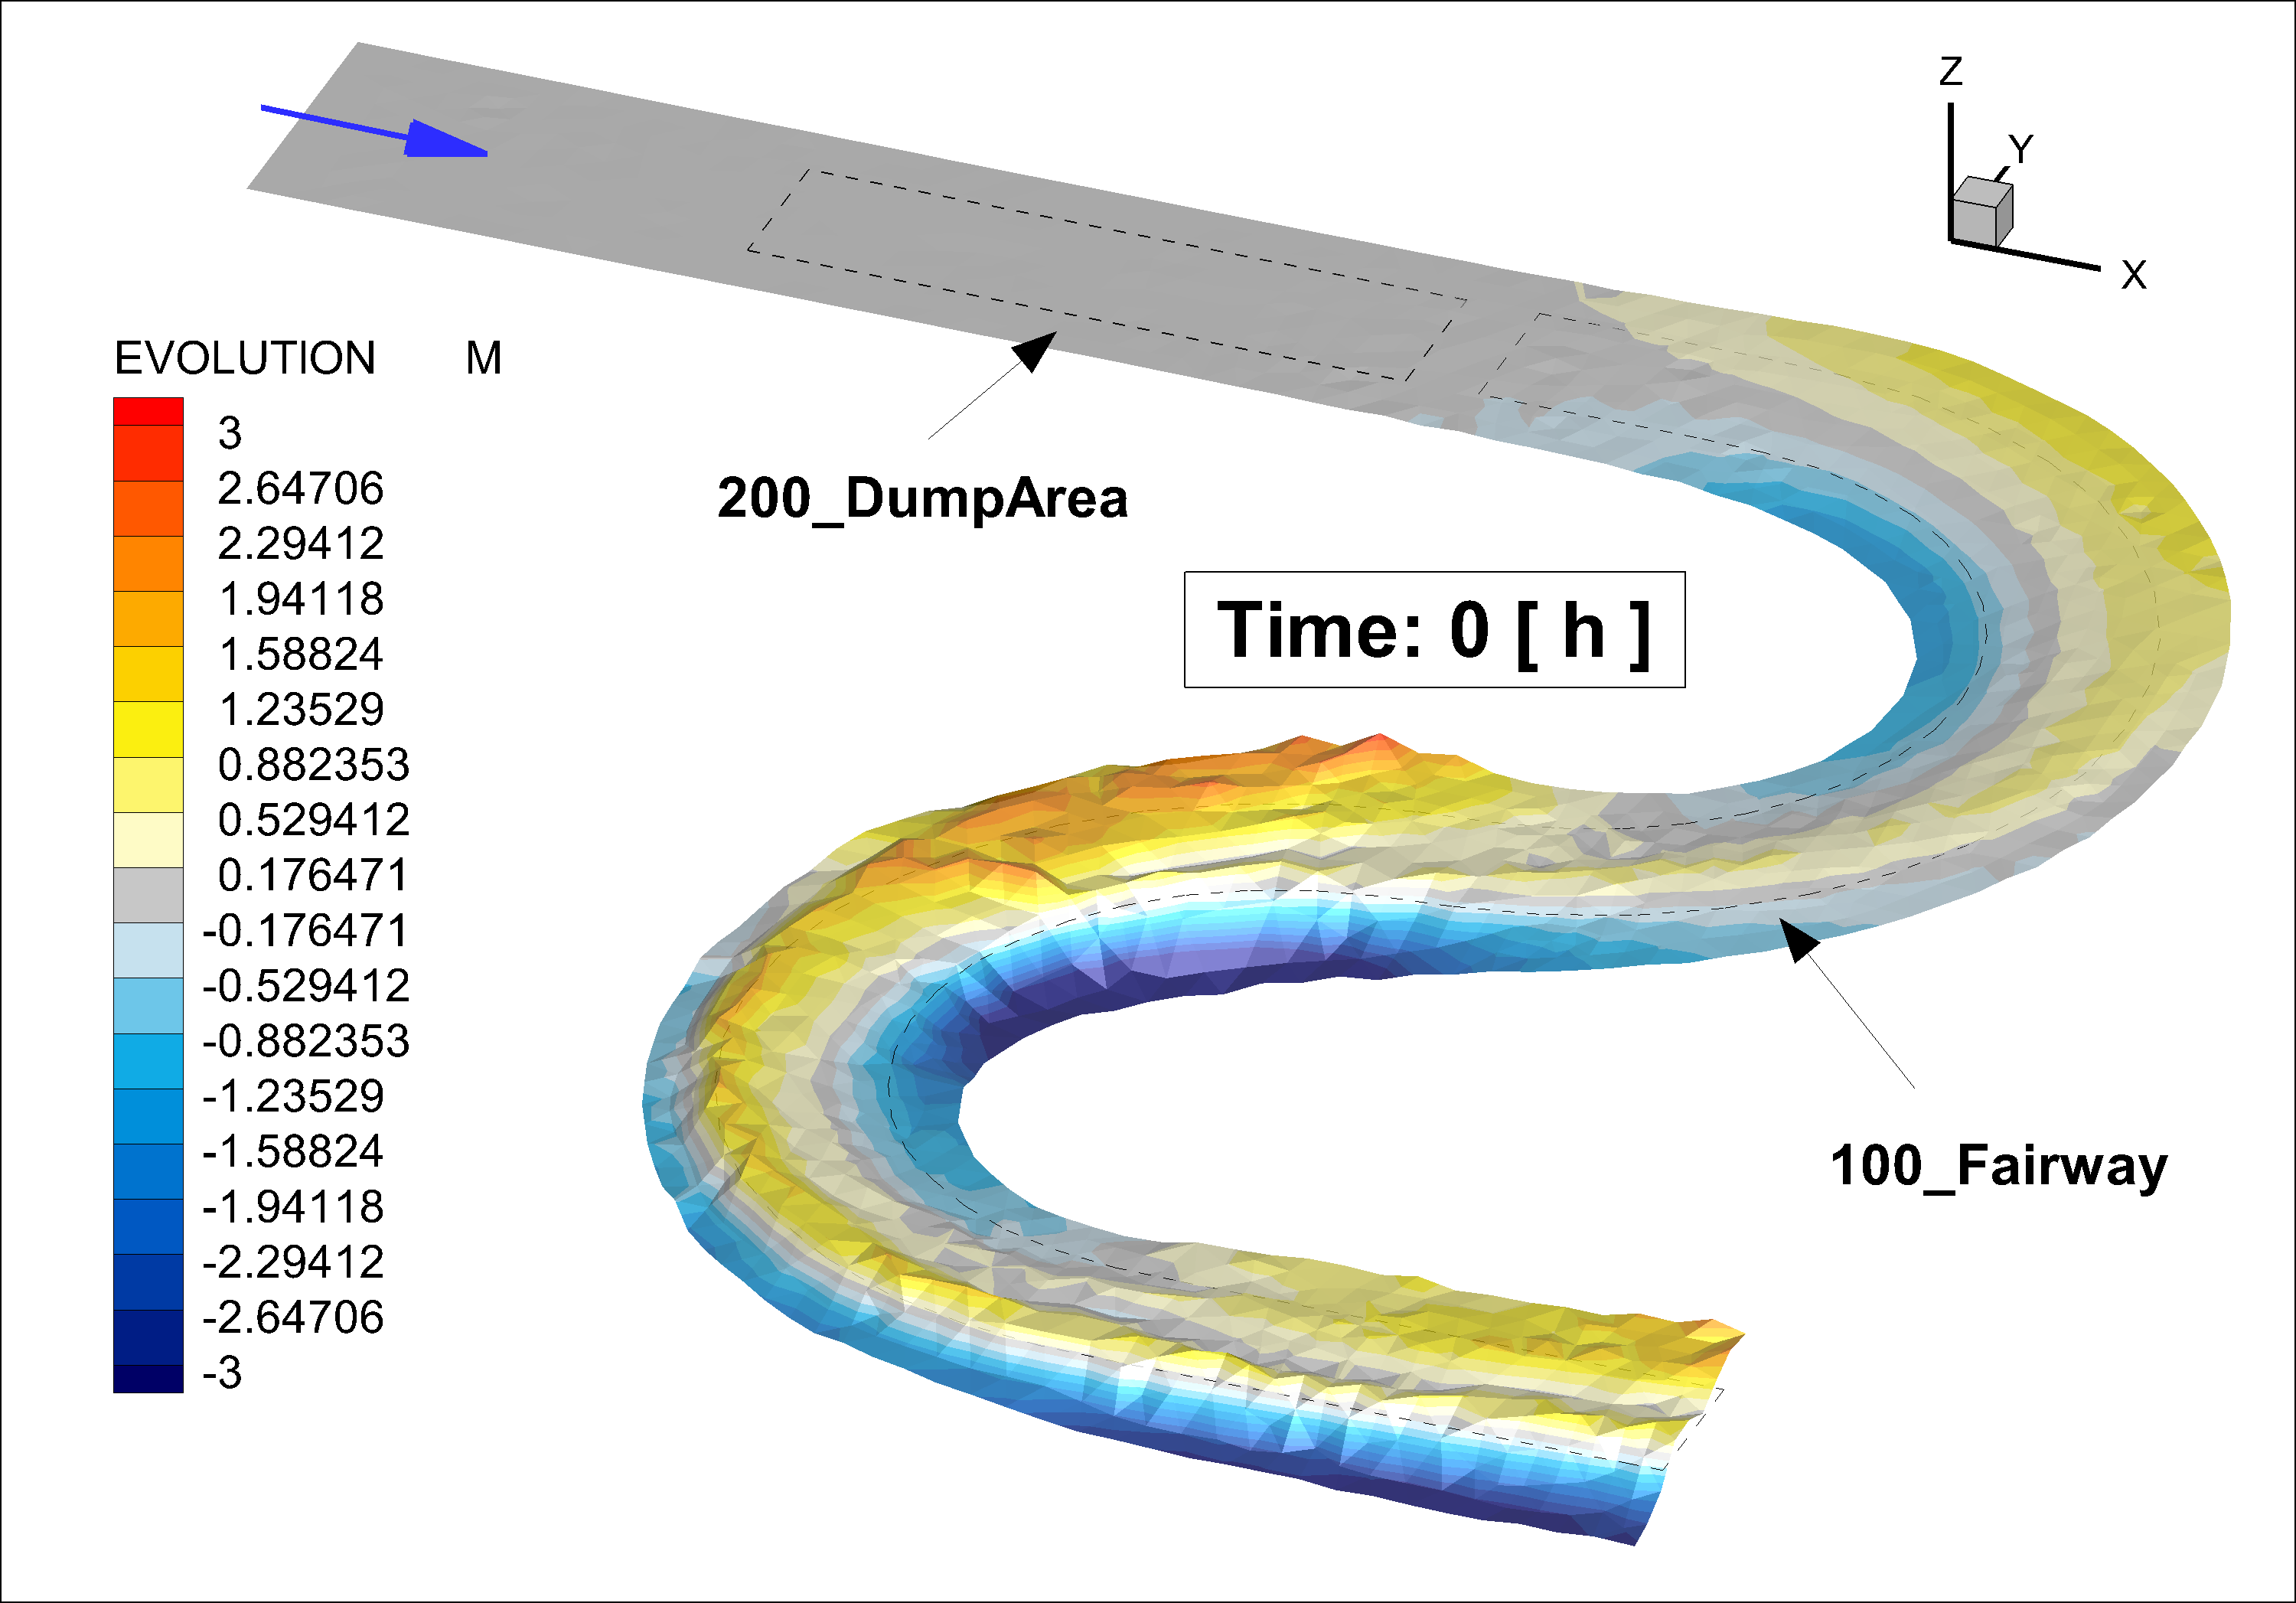
\includegraphics[scale=0.14]{../img/critDig_Poly_000h.png}
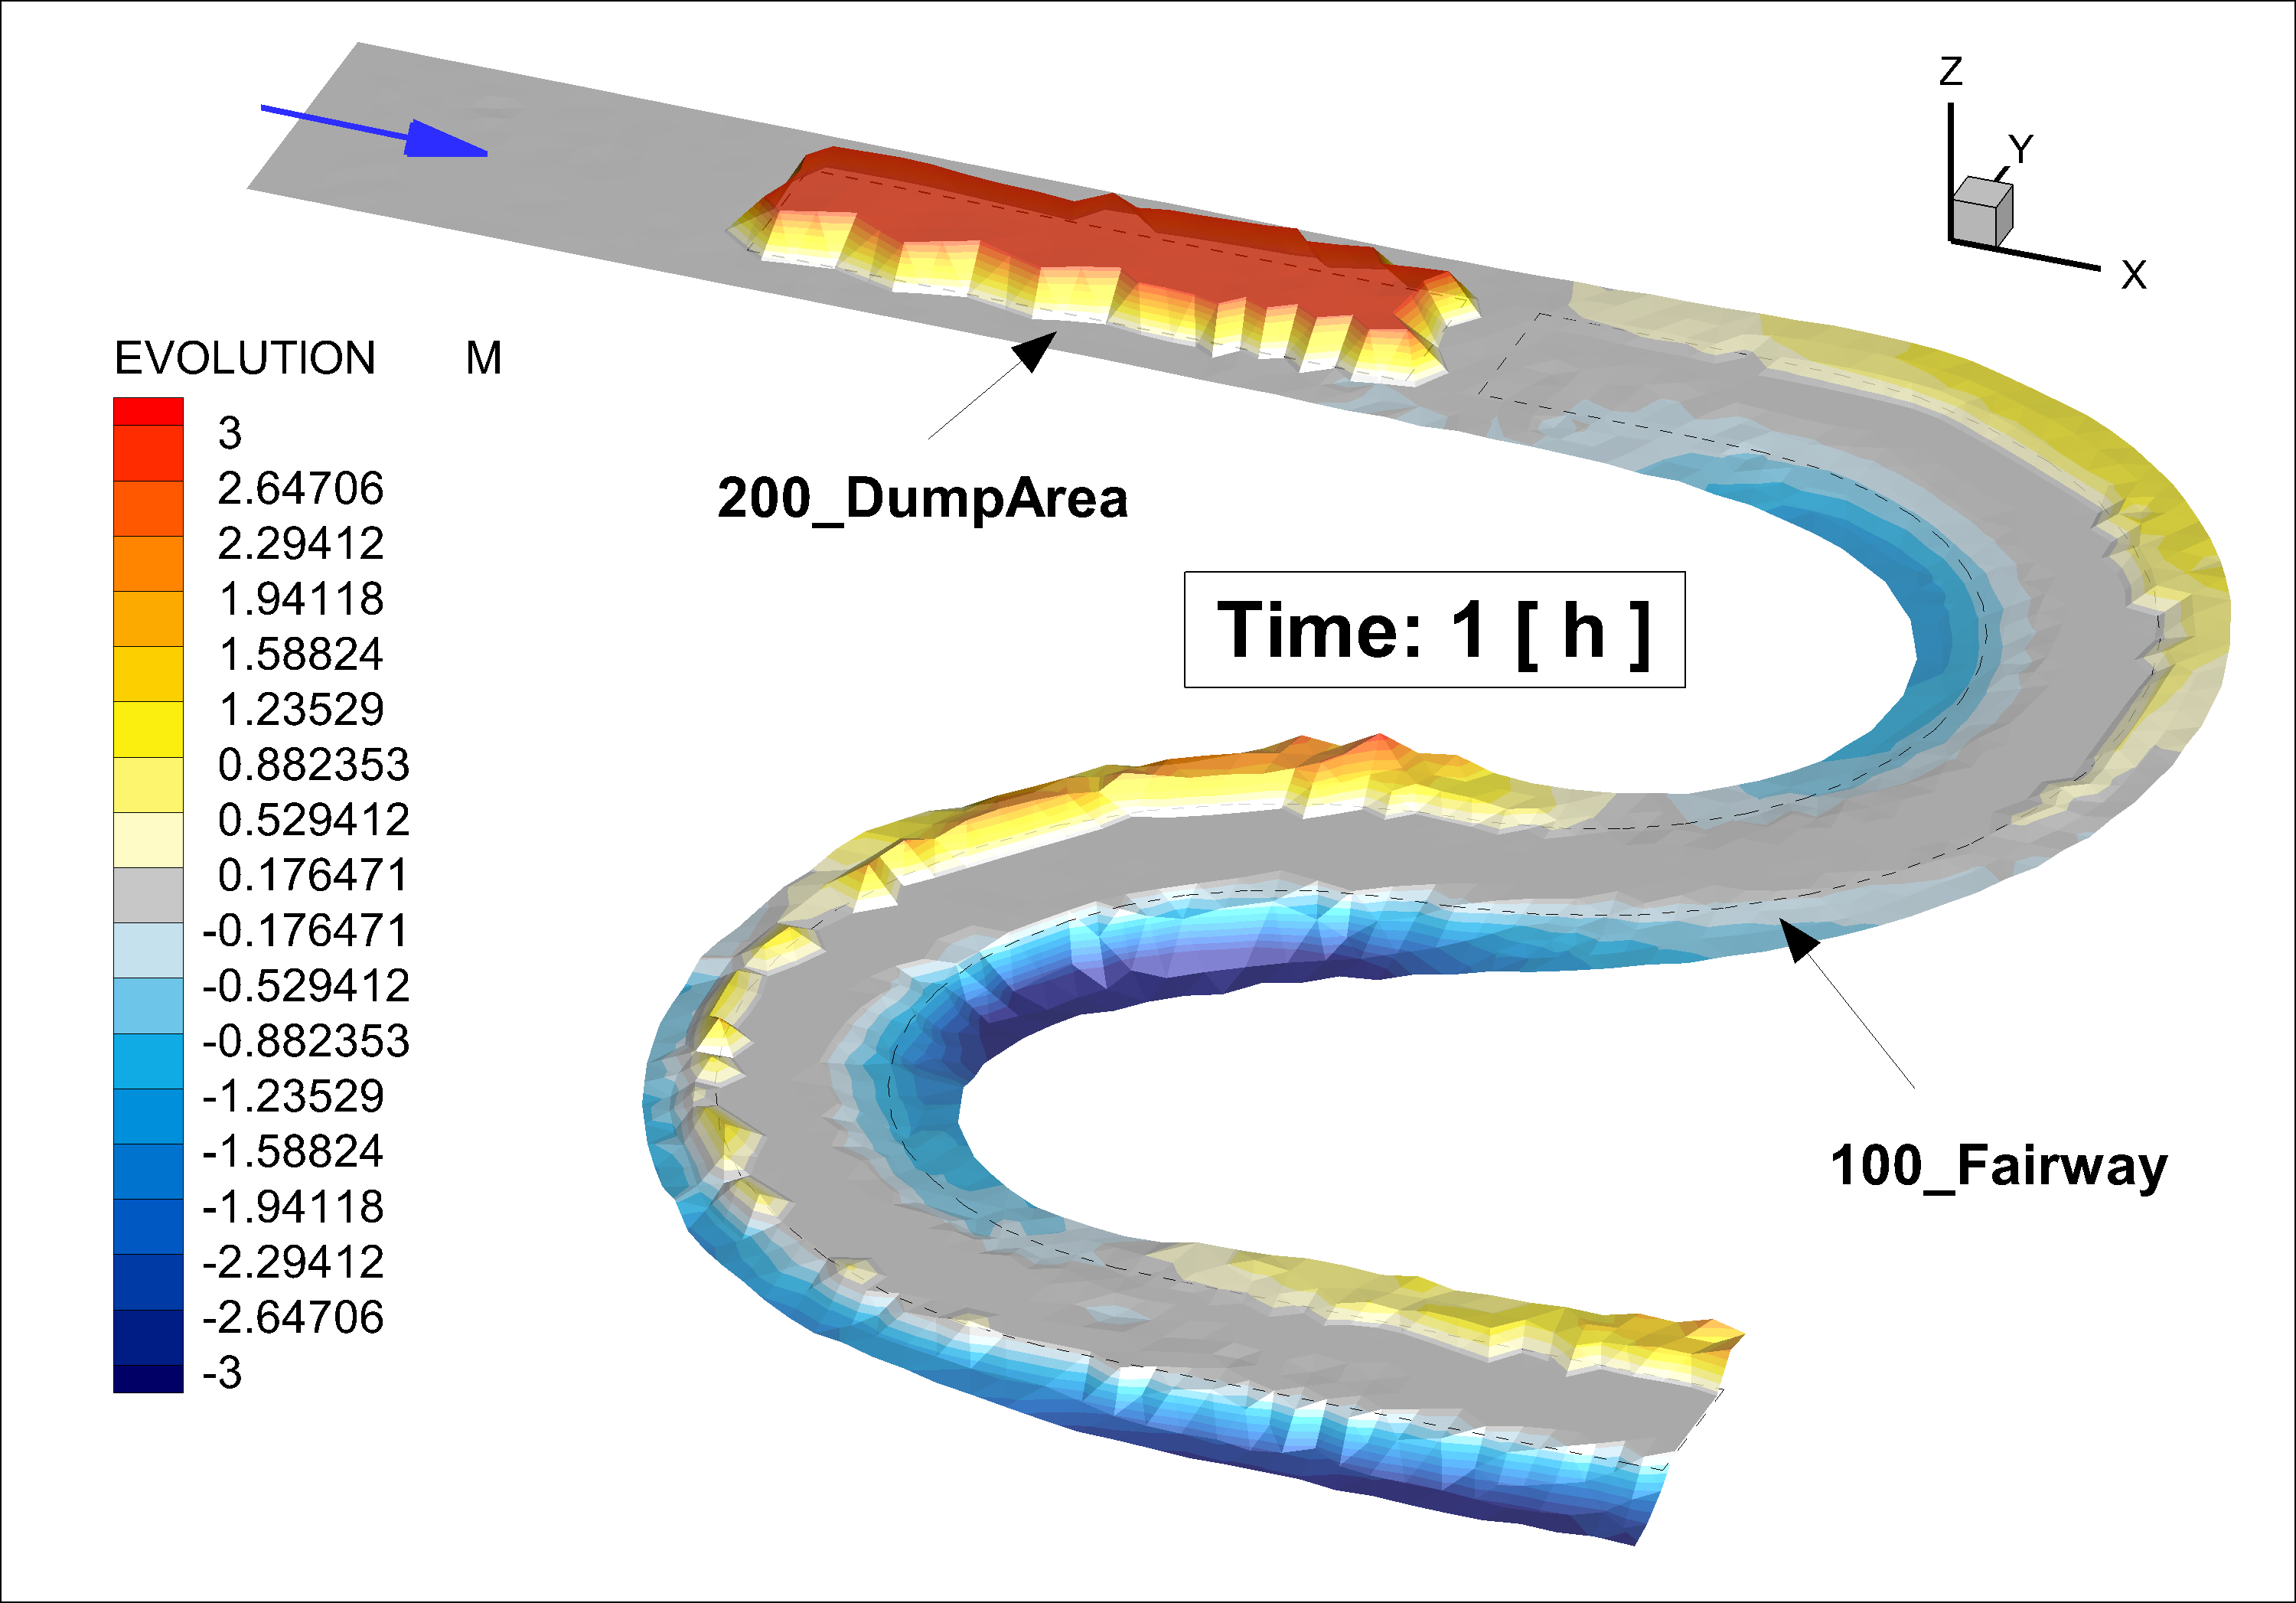
\includegraphics[scale=0.14]{../img/critDig_Poly_001h.png}
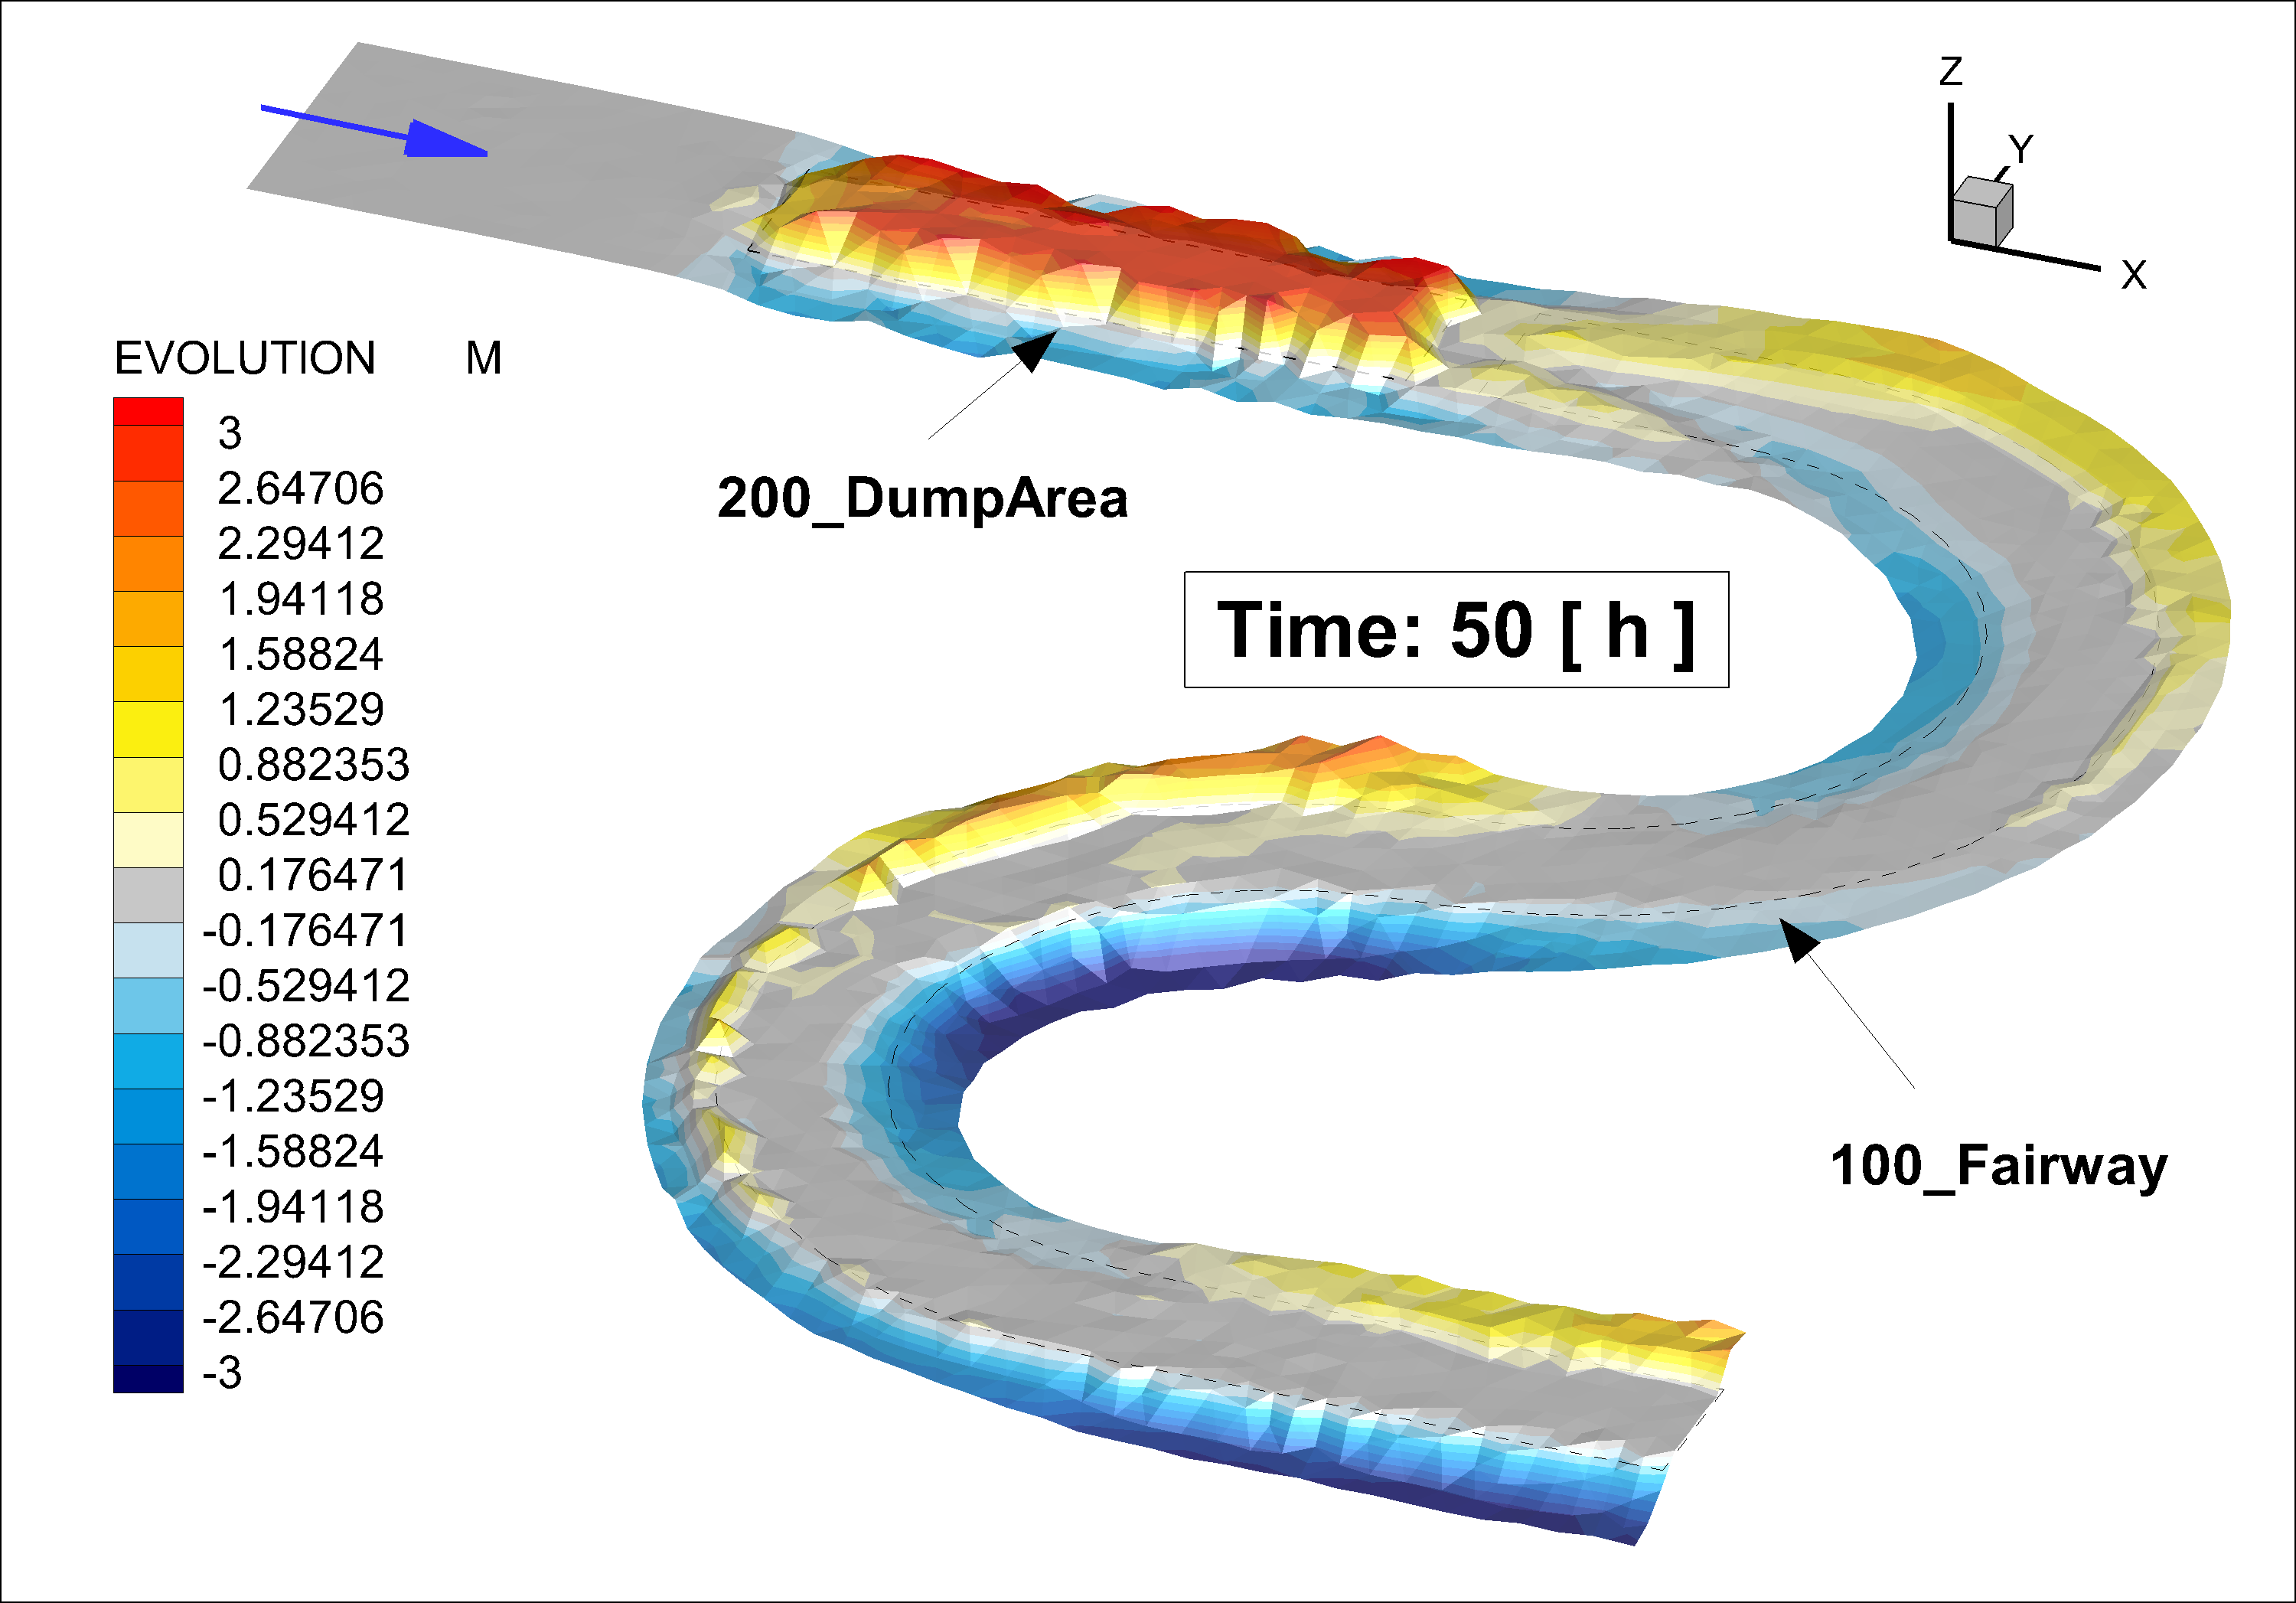
\includegraphics[scale=0.14]{../img/critDig_Poly_050h.png}
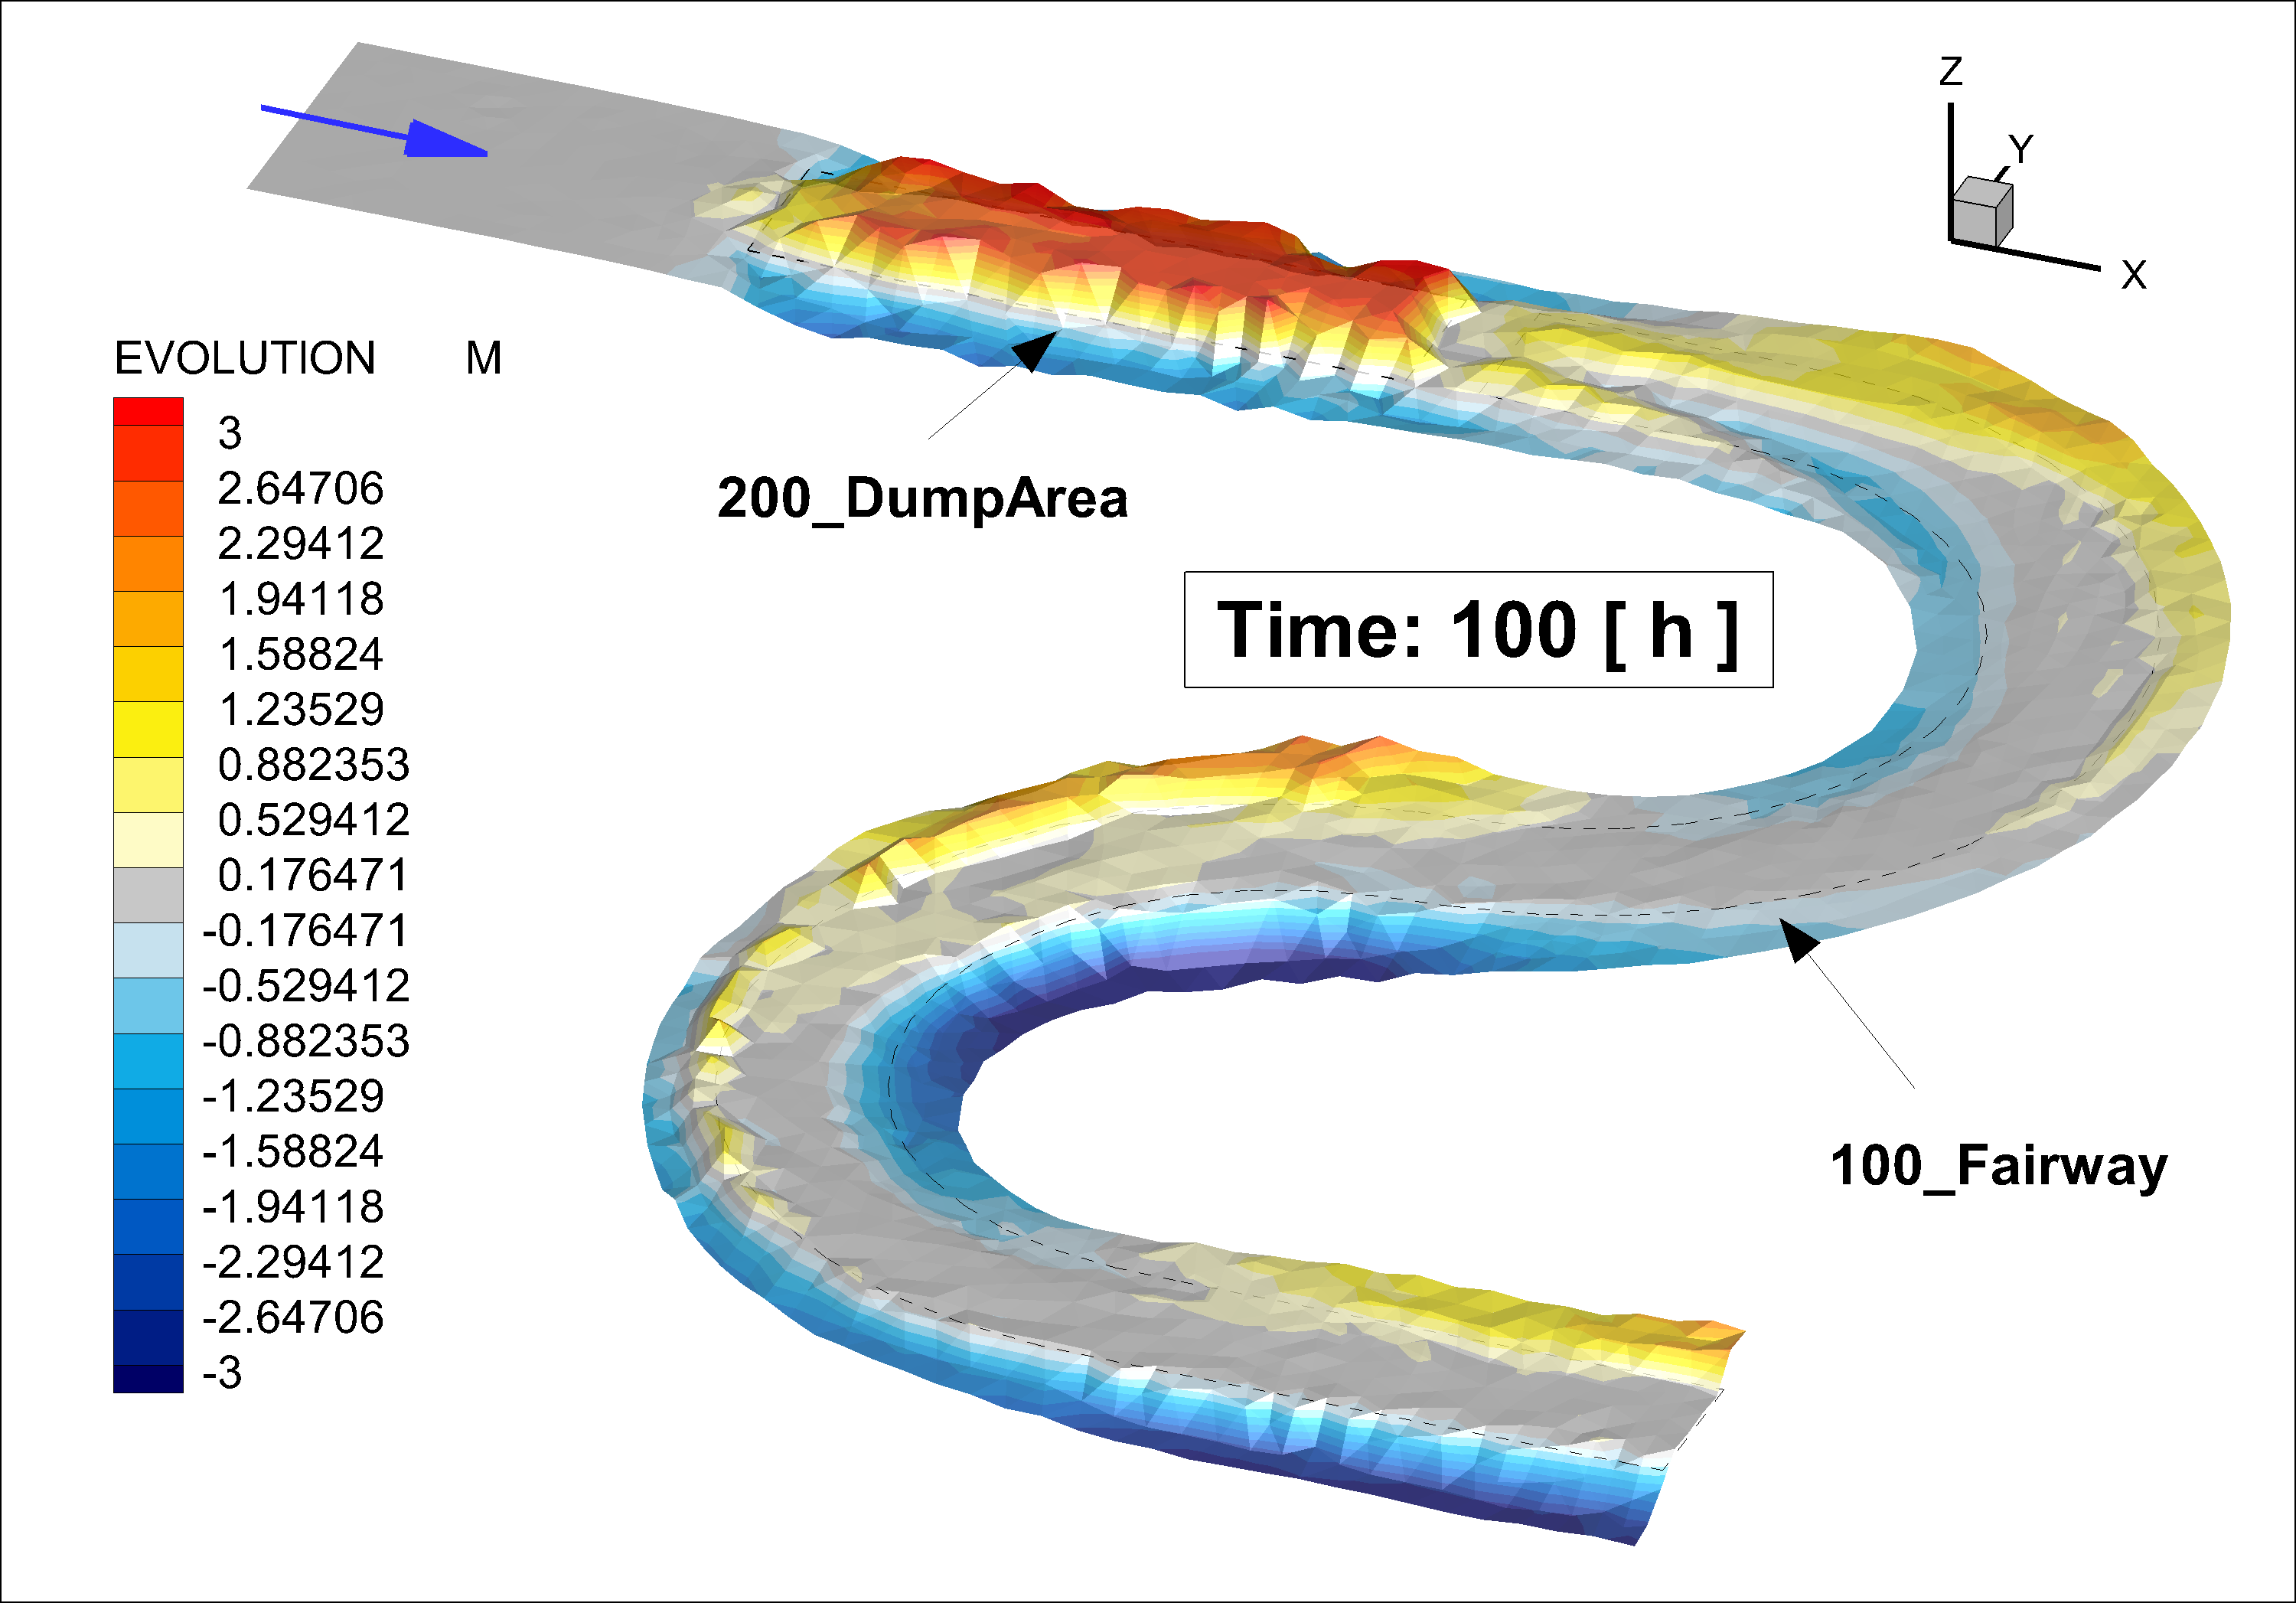
\includegraphics[scale=0.14]{../img/critDig_Poly_100h.png}
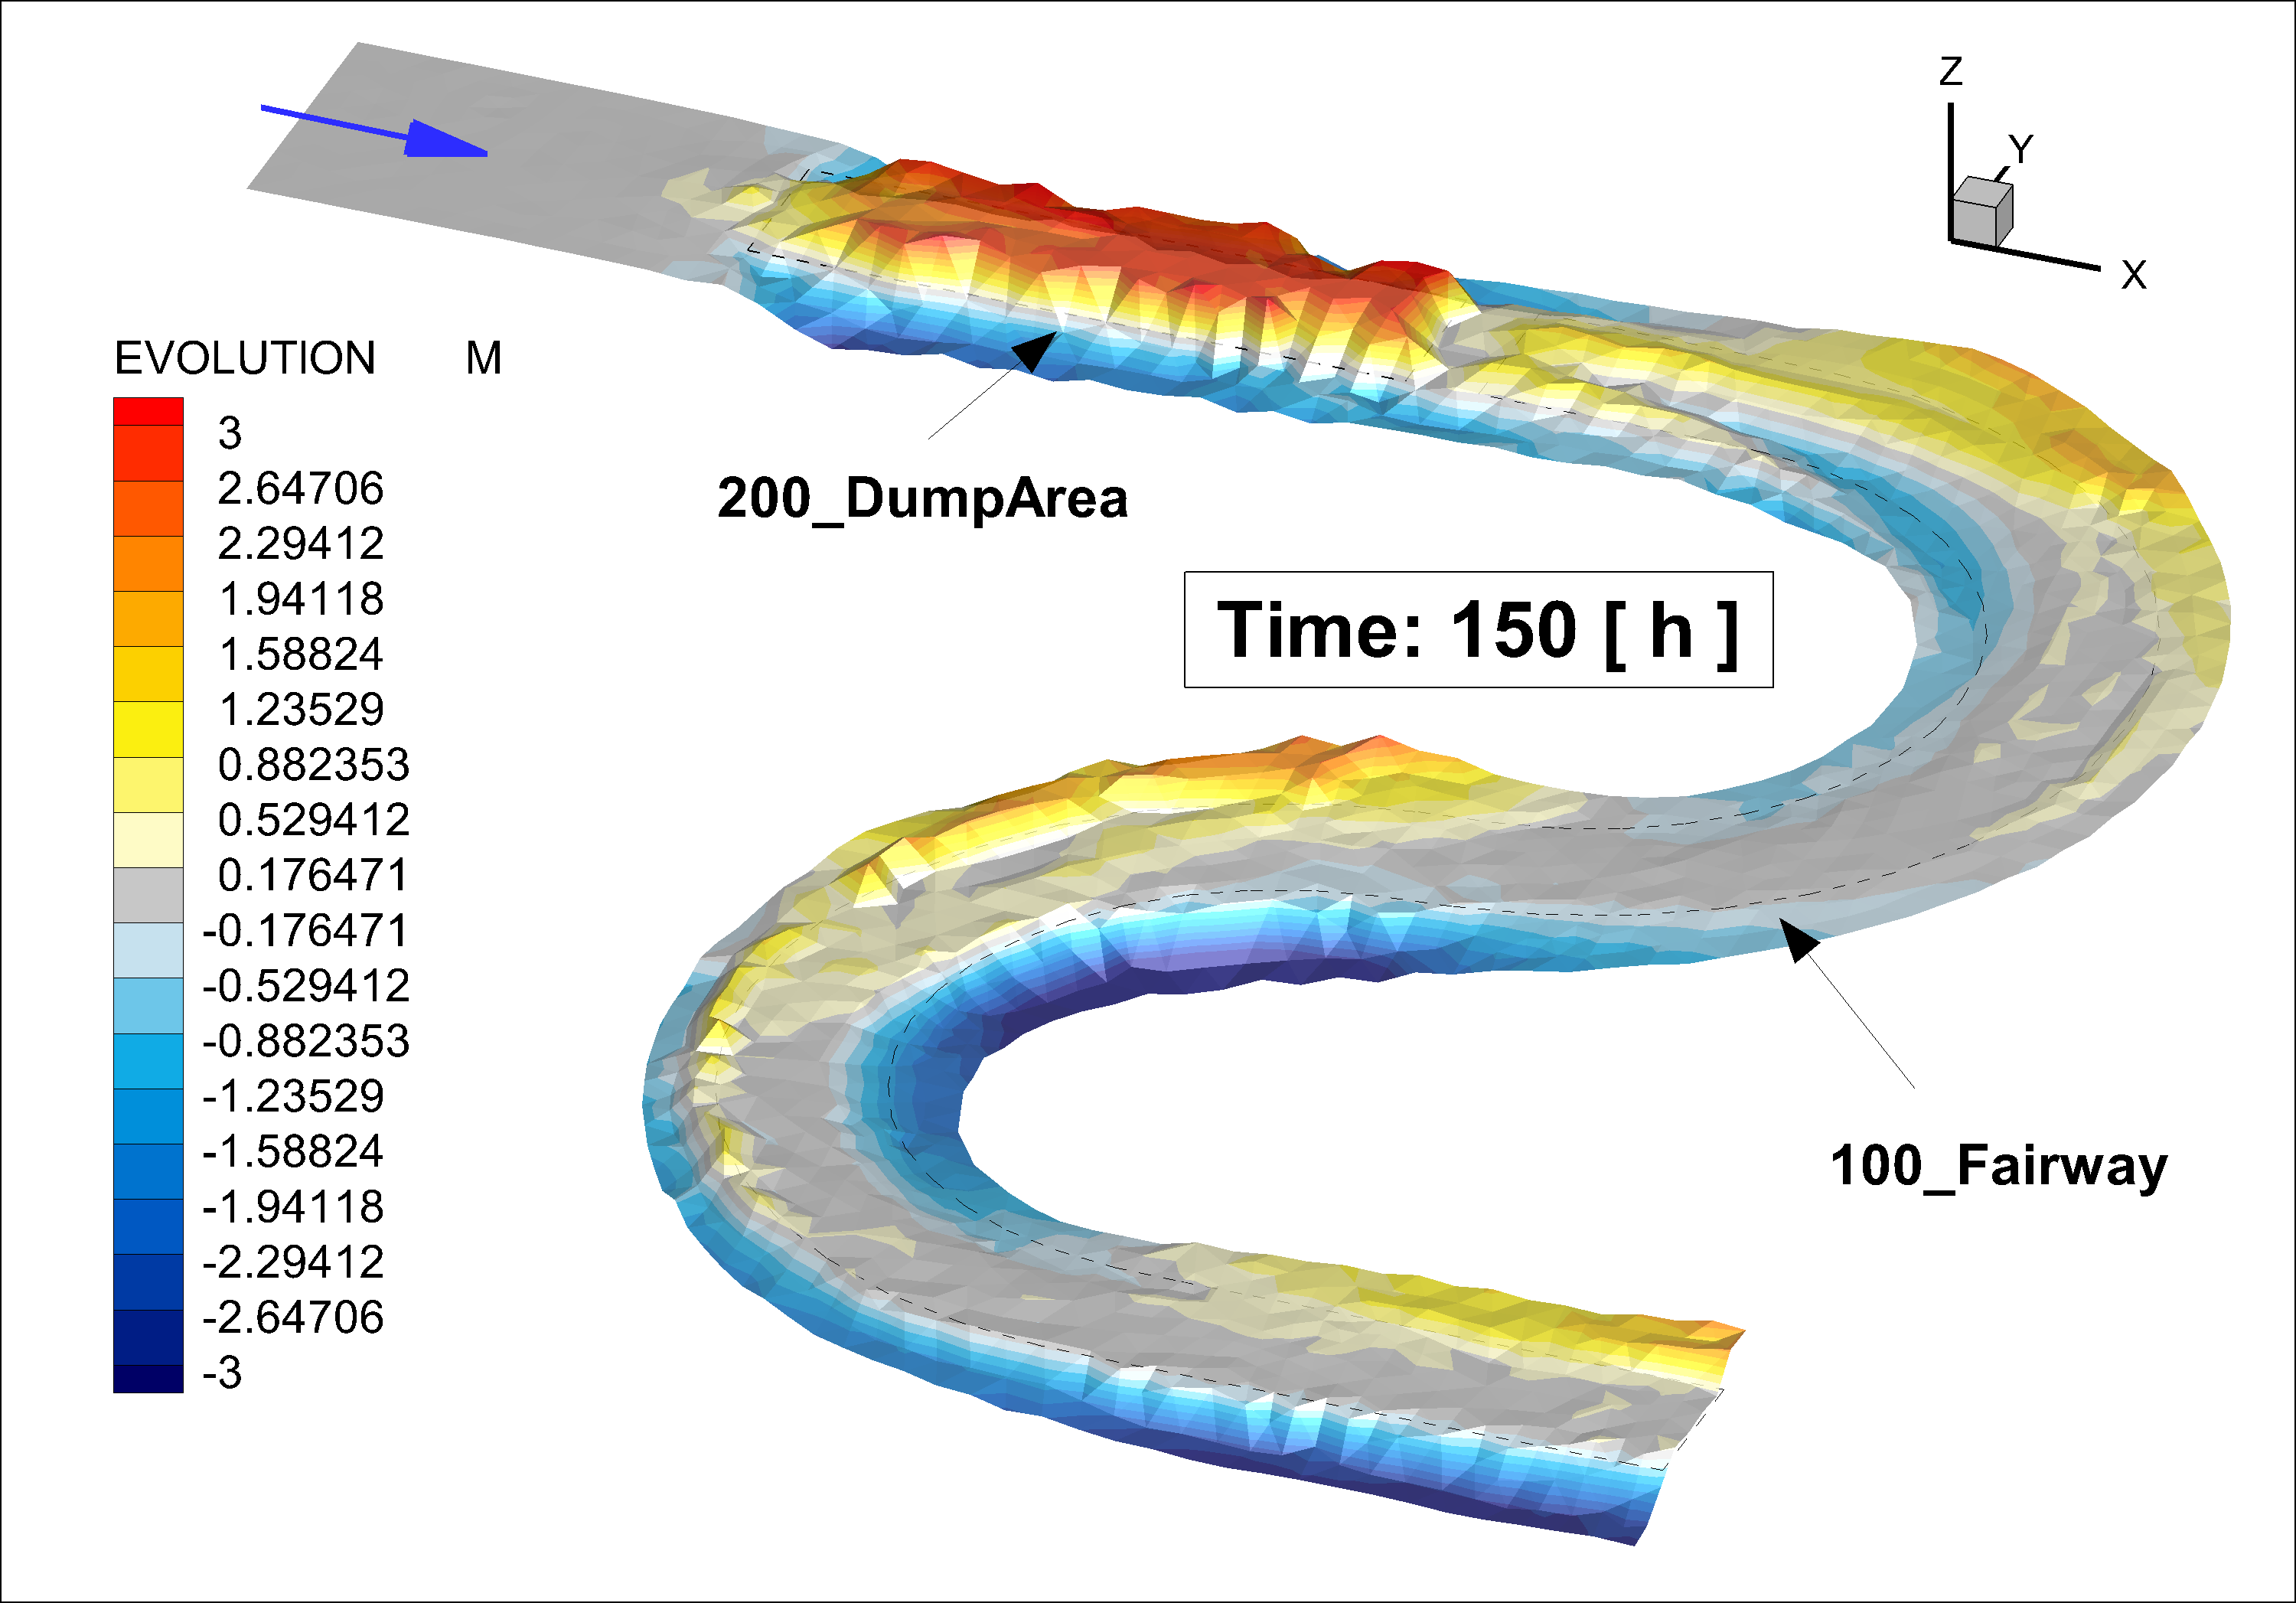
\includegraphics[scale=0.14]{../img/critDig_Poly_150h.png}
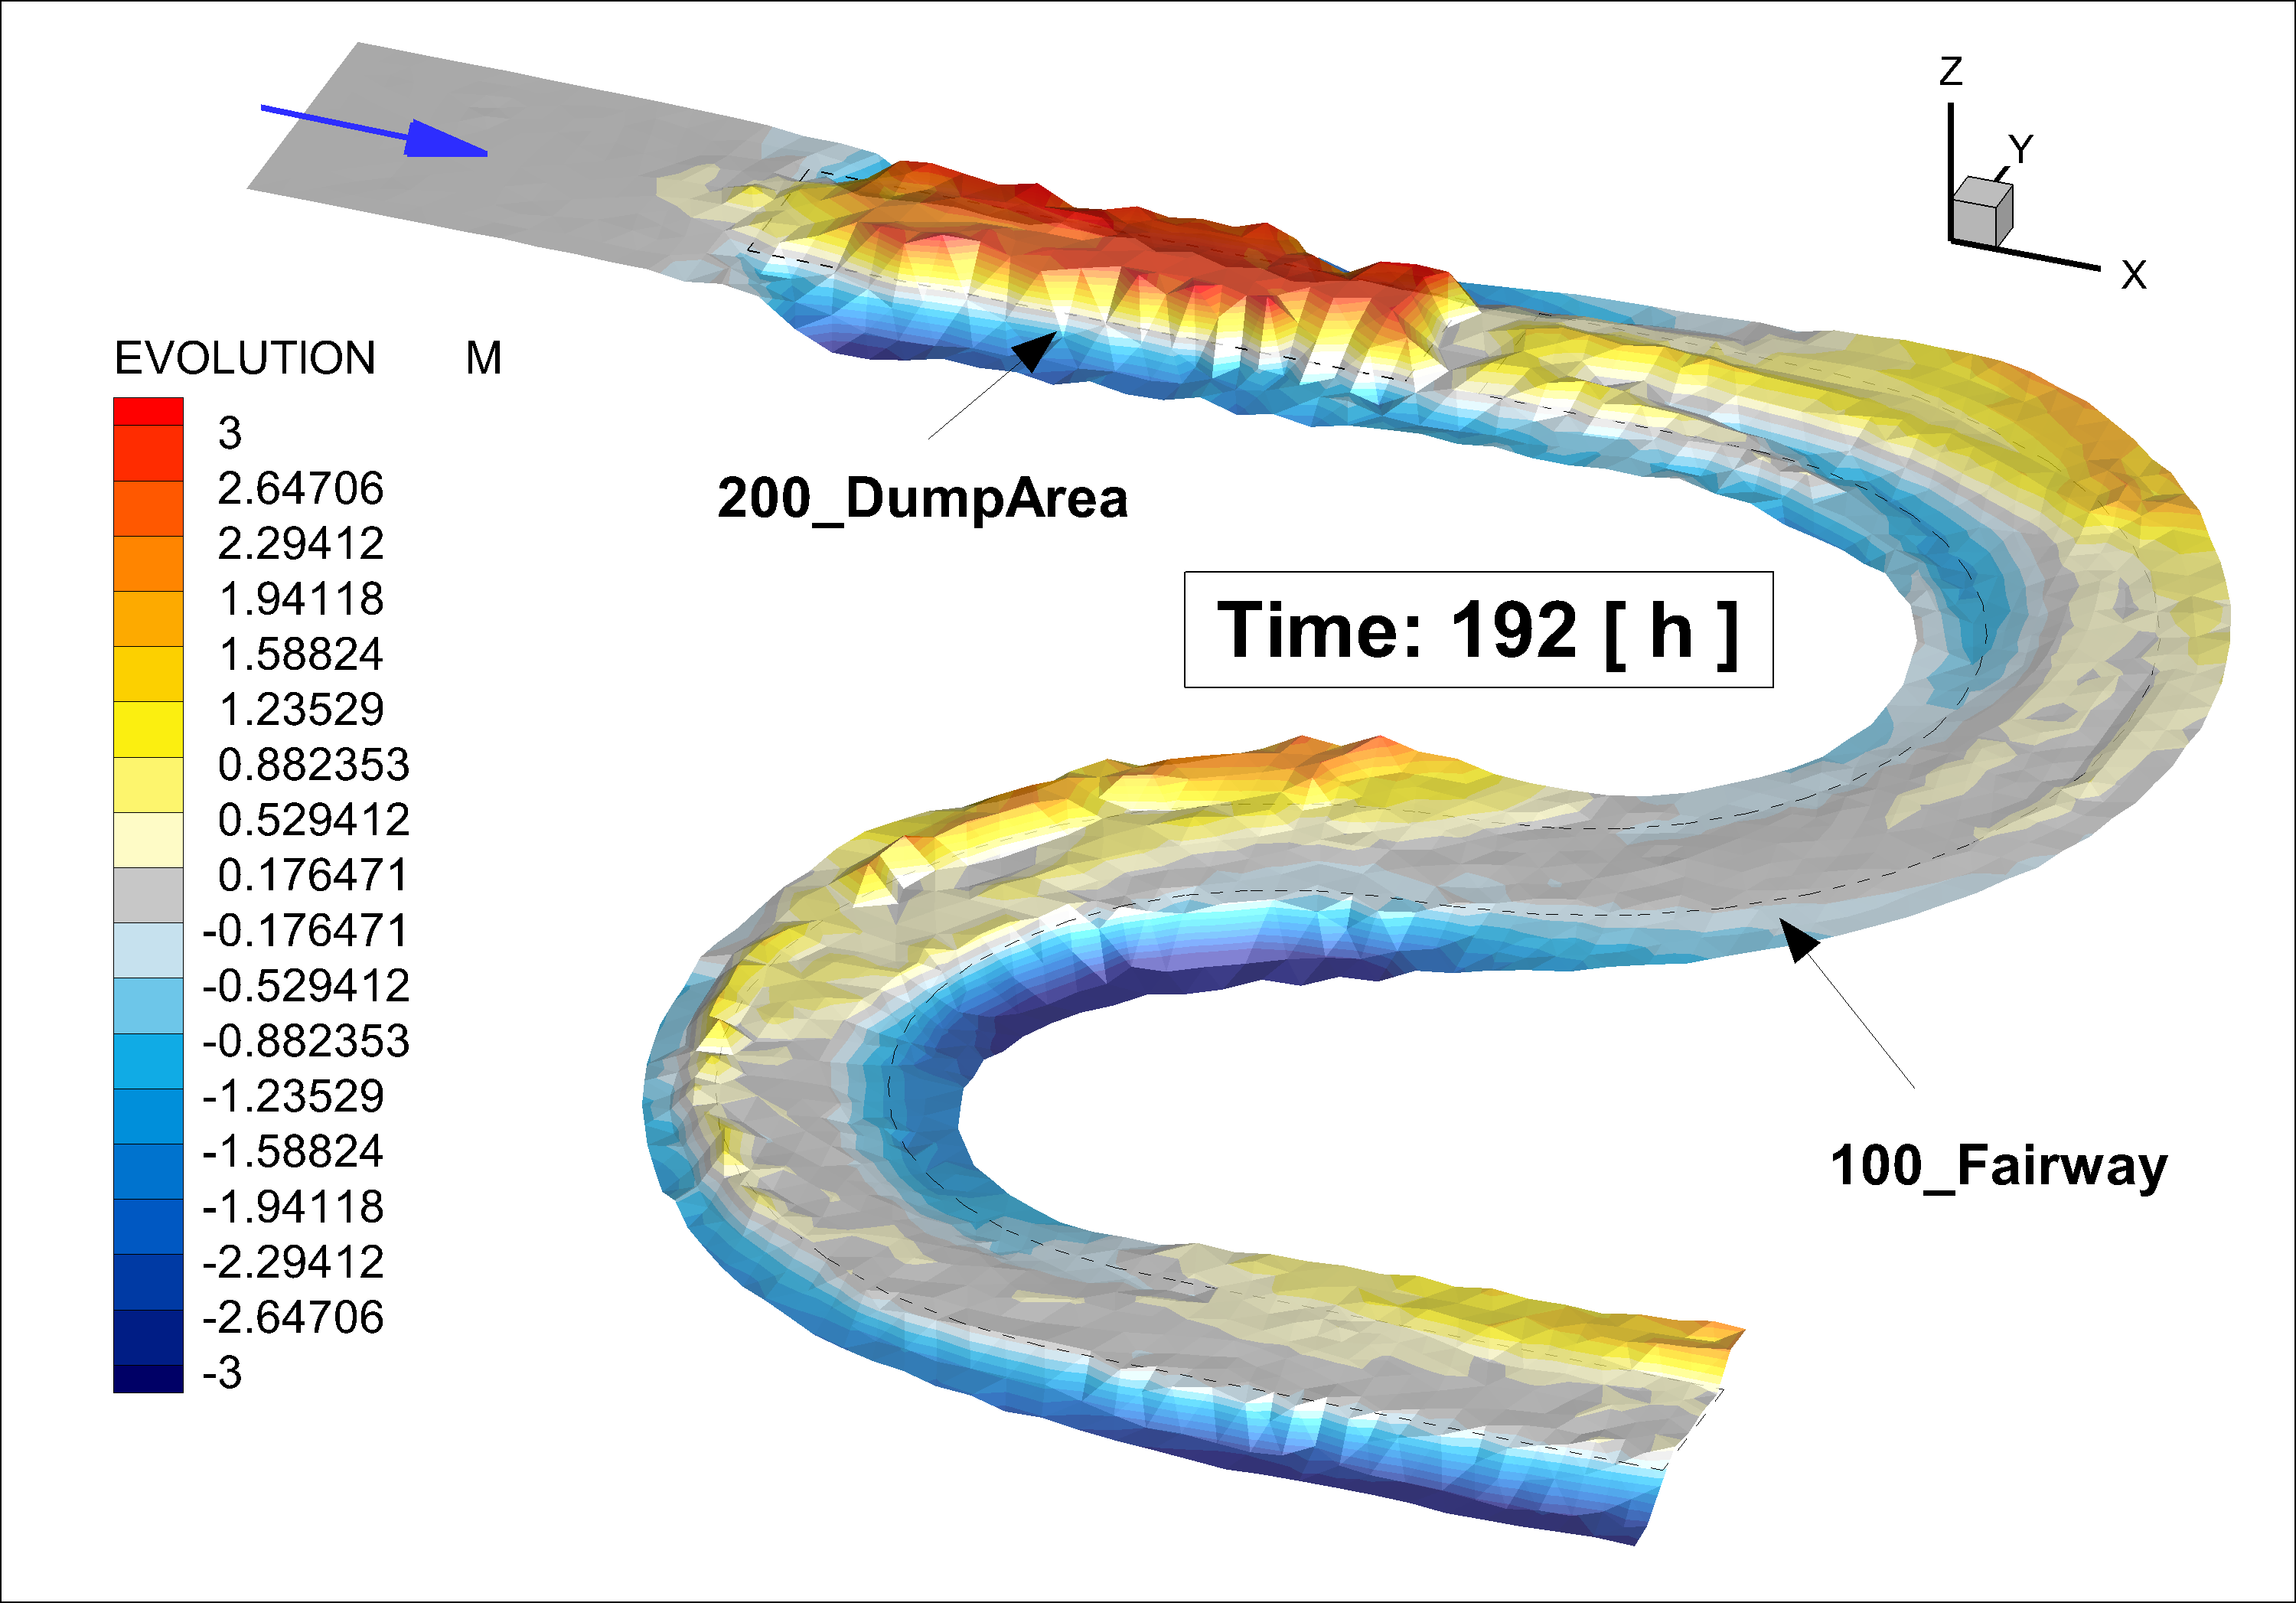
\includegraphics[scale=0.14]{../img/critDig_Poly_192h.png}
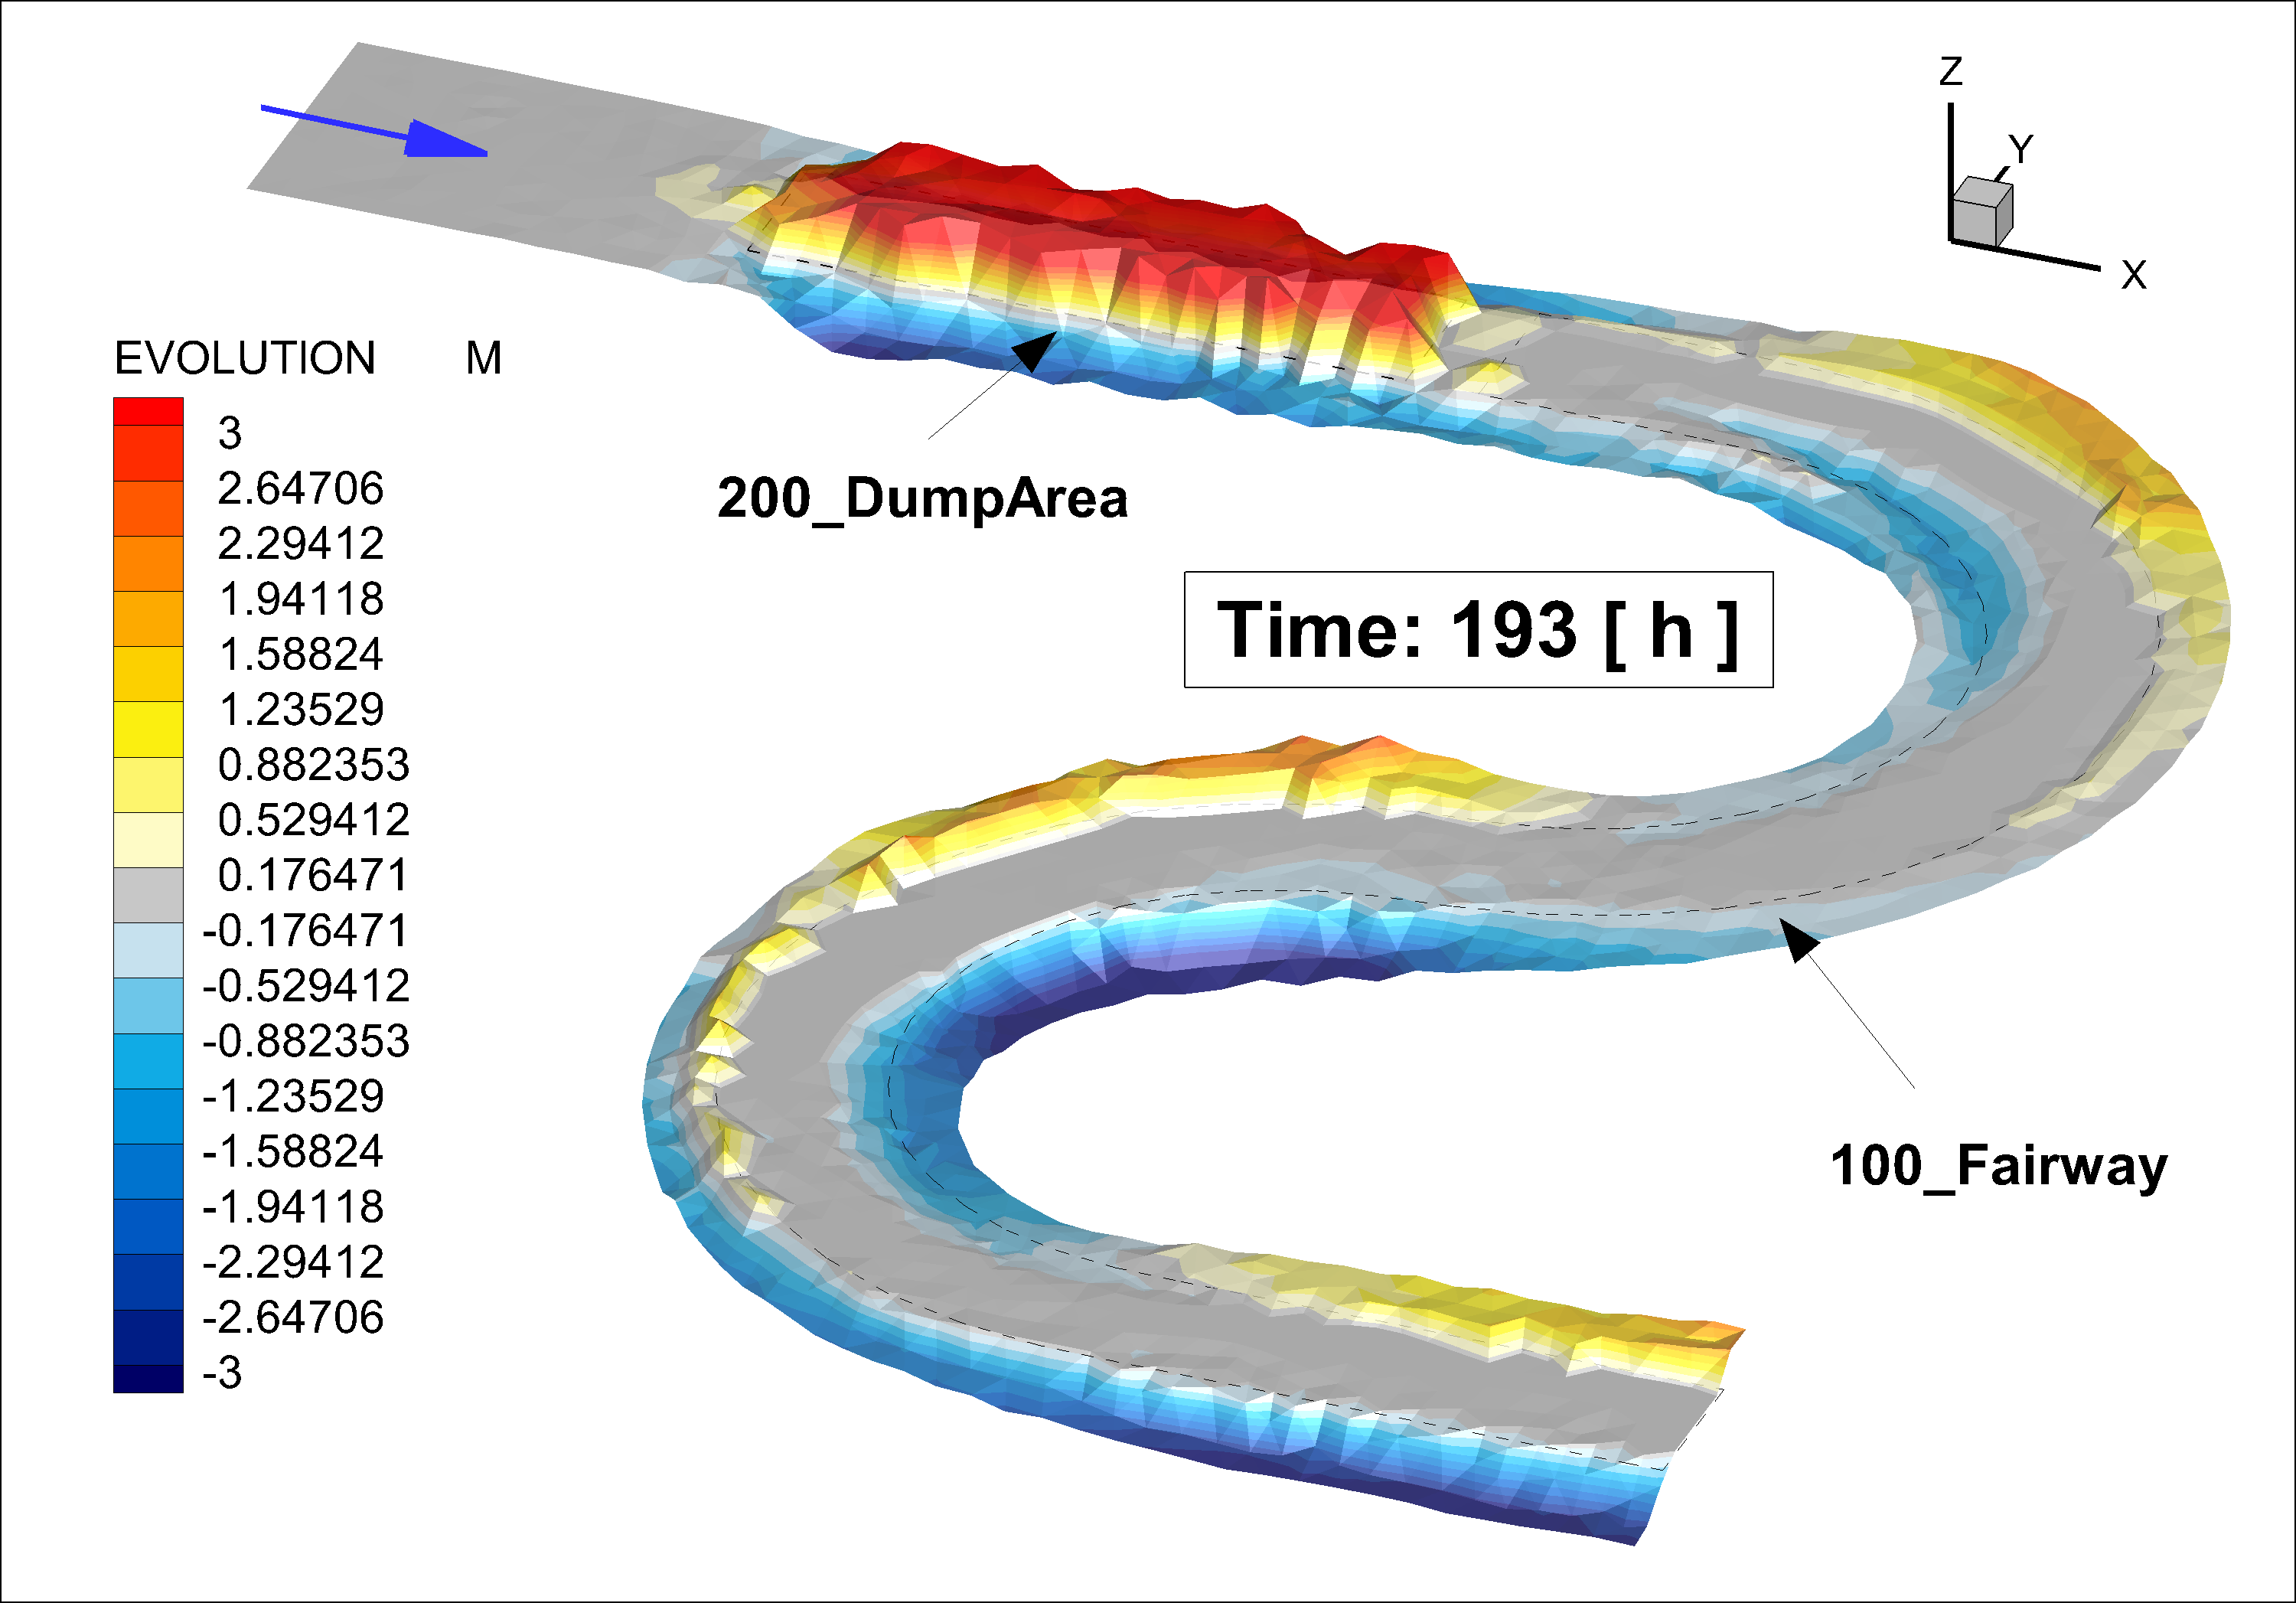
\includegraphics[scale=0.14]{../img/critDig_Poly_193h.png}
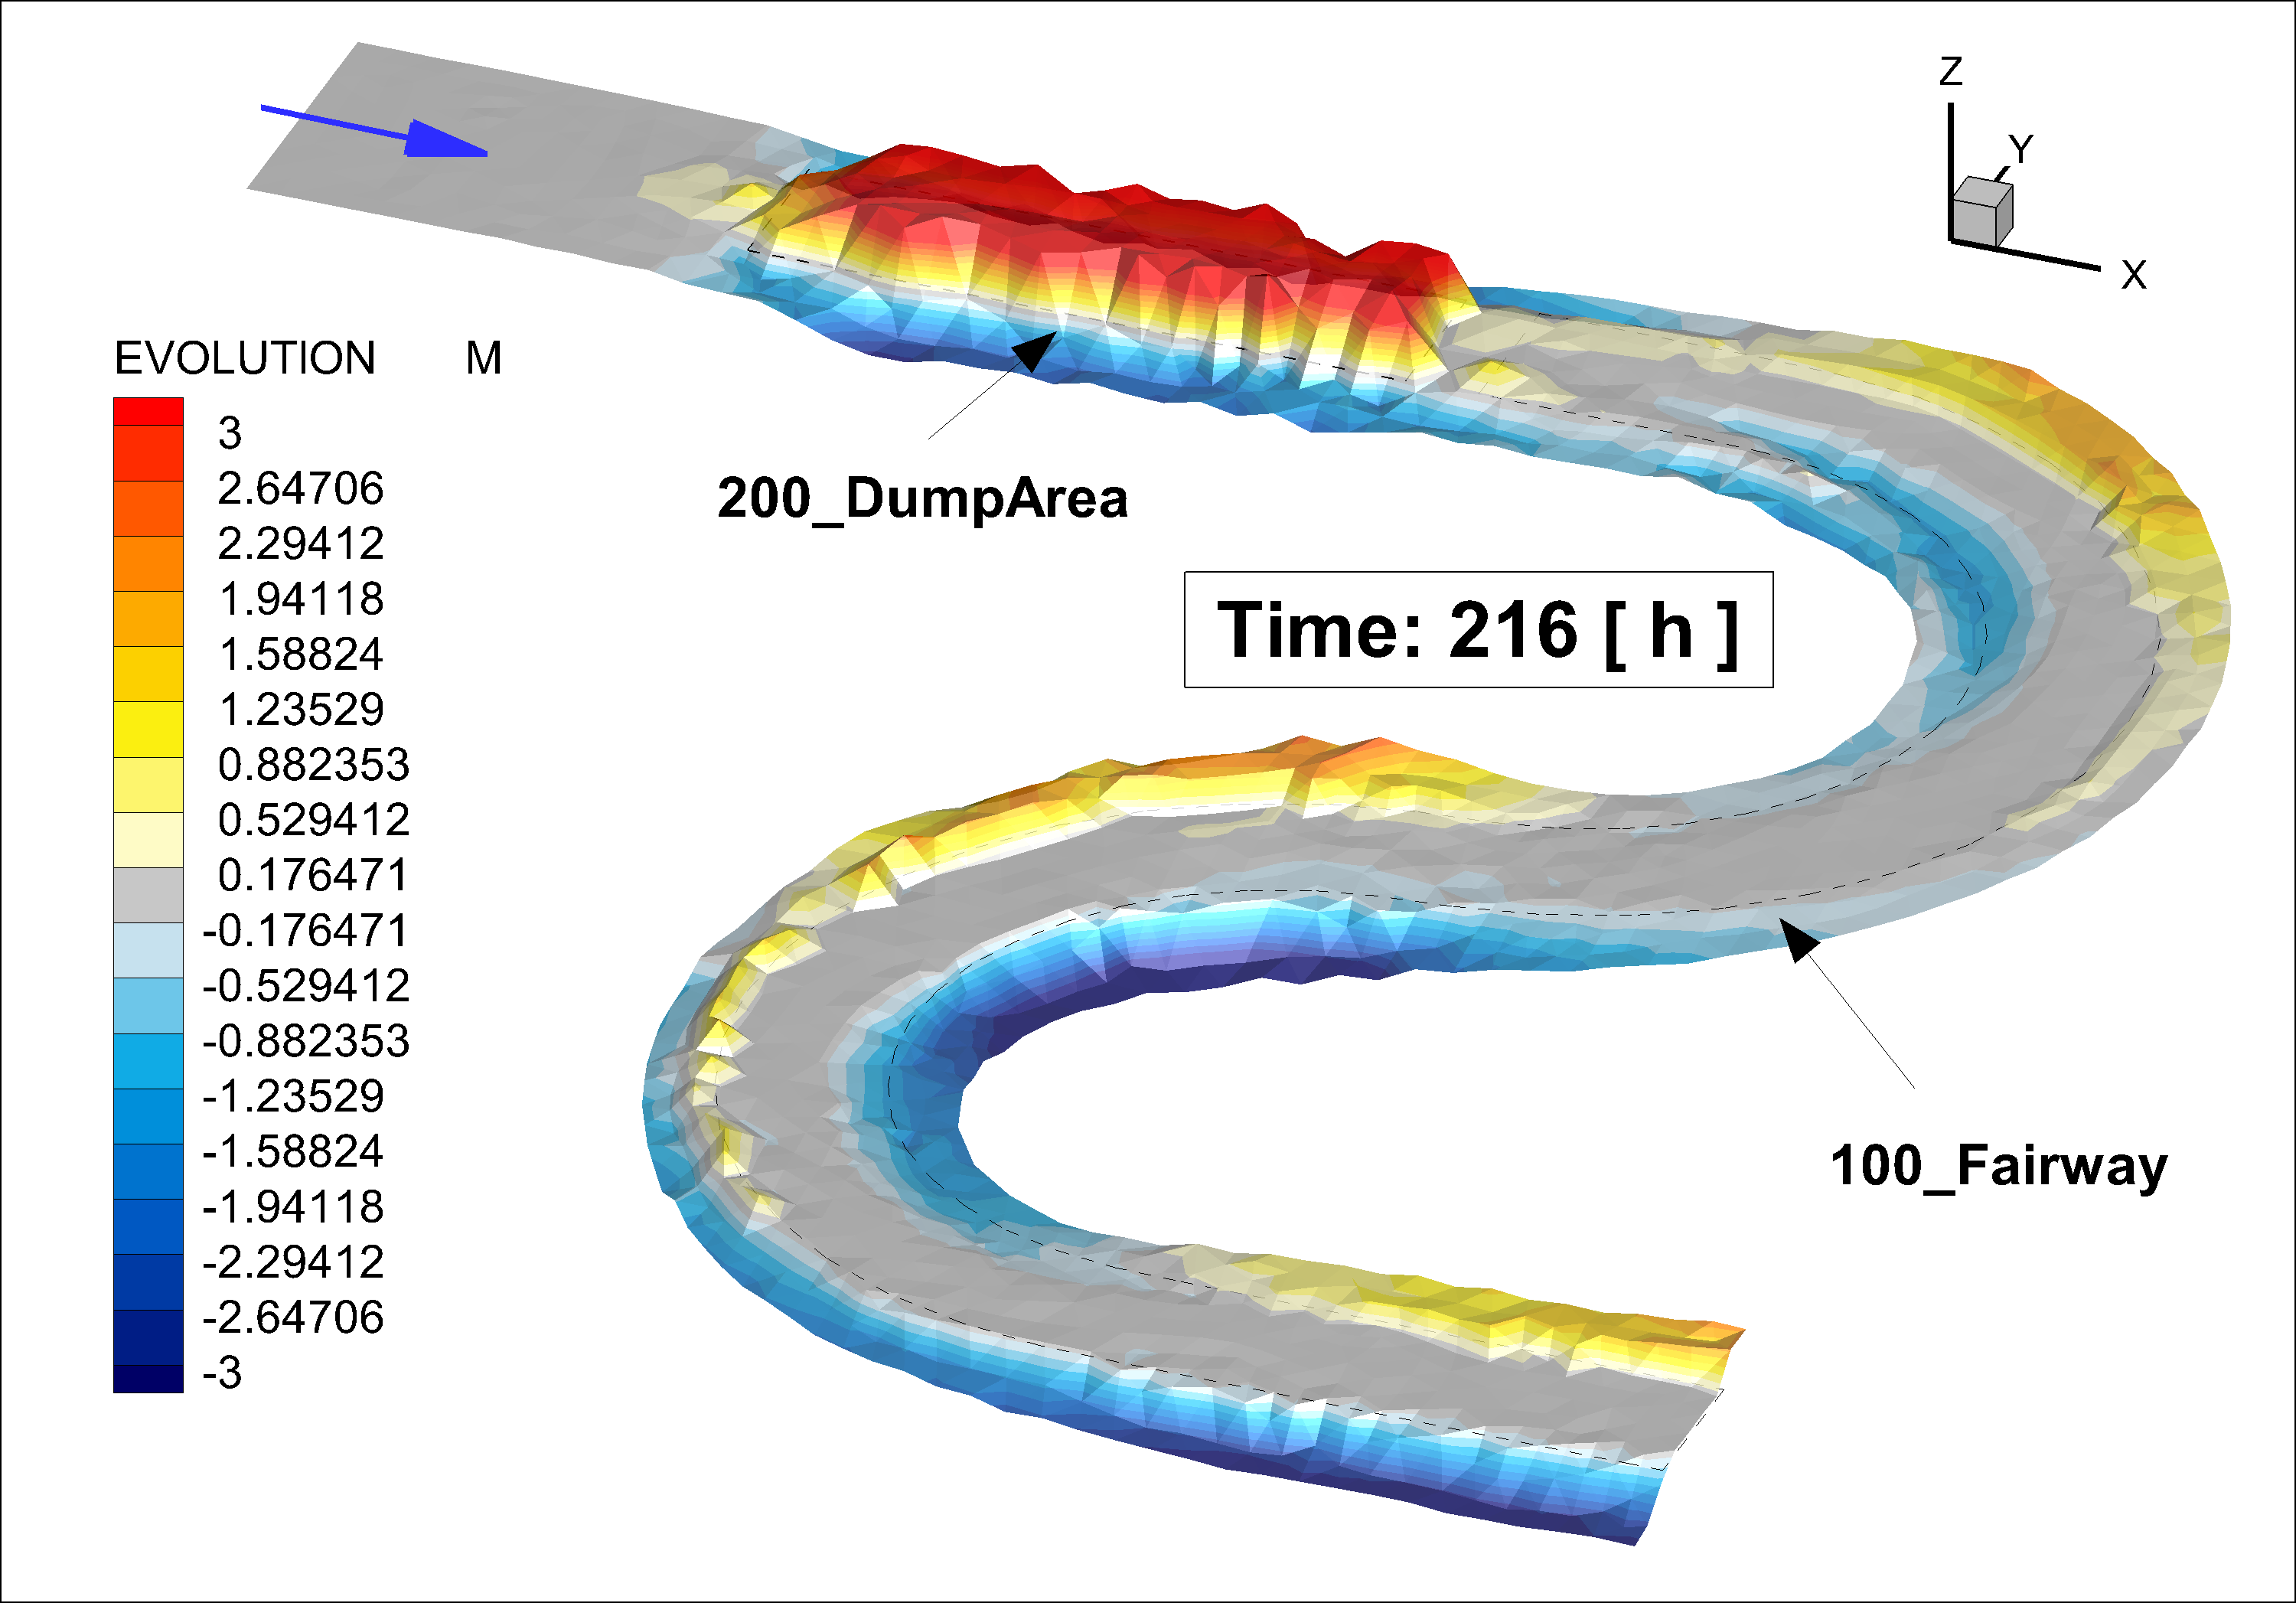
\includegraphics[scale=0.14]{../img/critDig_Poly_216h.png}
\caption{Simulated evolution over the time.}\label{result50}
\end{figure}

%Figure \ref{result3D} shows the evolution after 0s and 150s as 3D view. 
%\begin{figure} [!h]
%\centering
%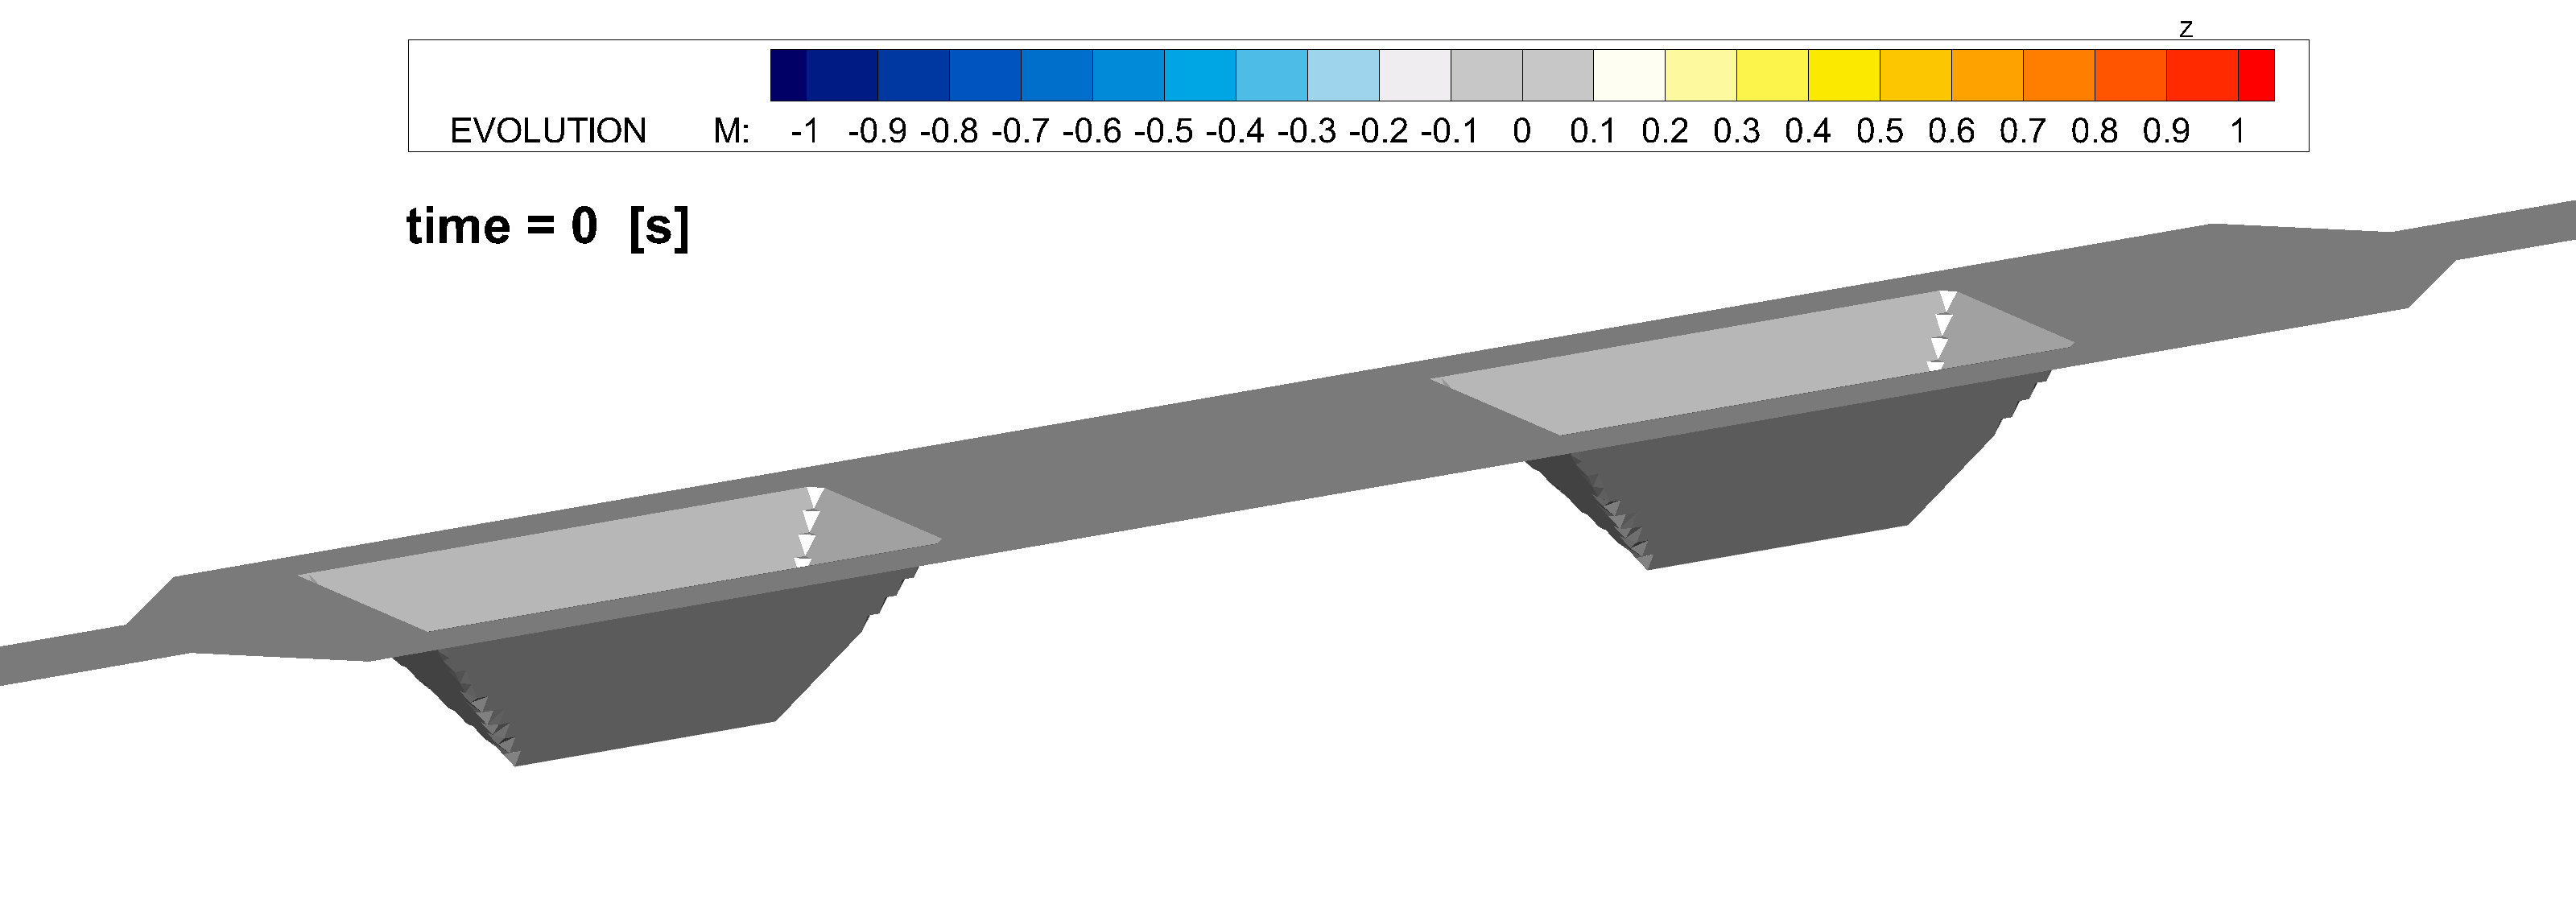
\includegraphics[scale=0.14]{../img/result000_zoom3D.png}
%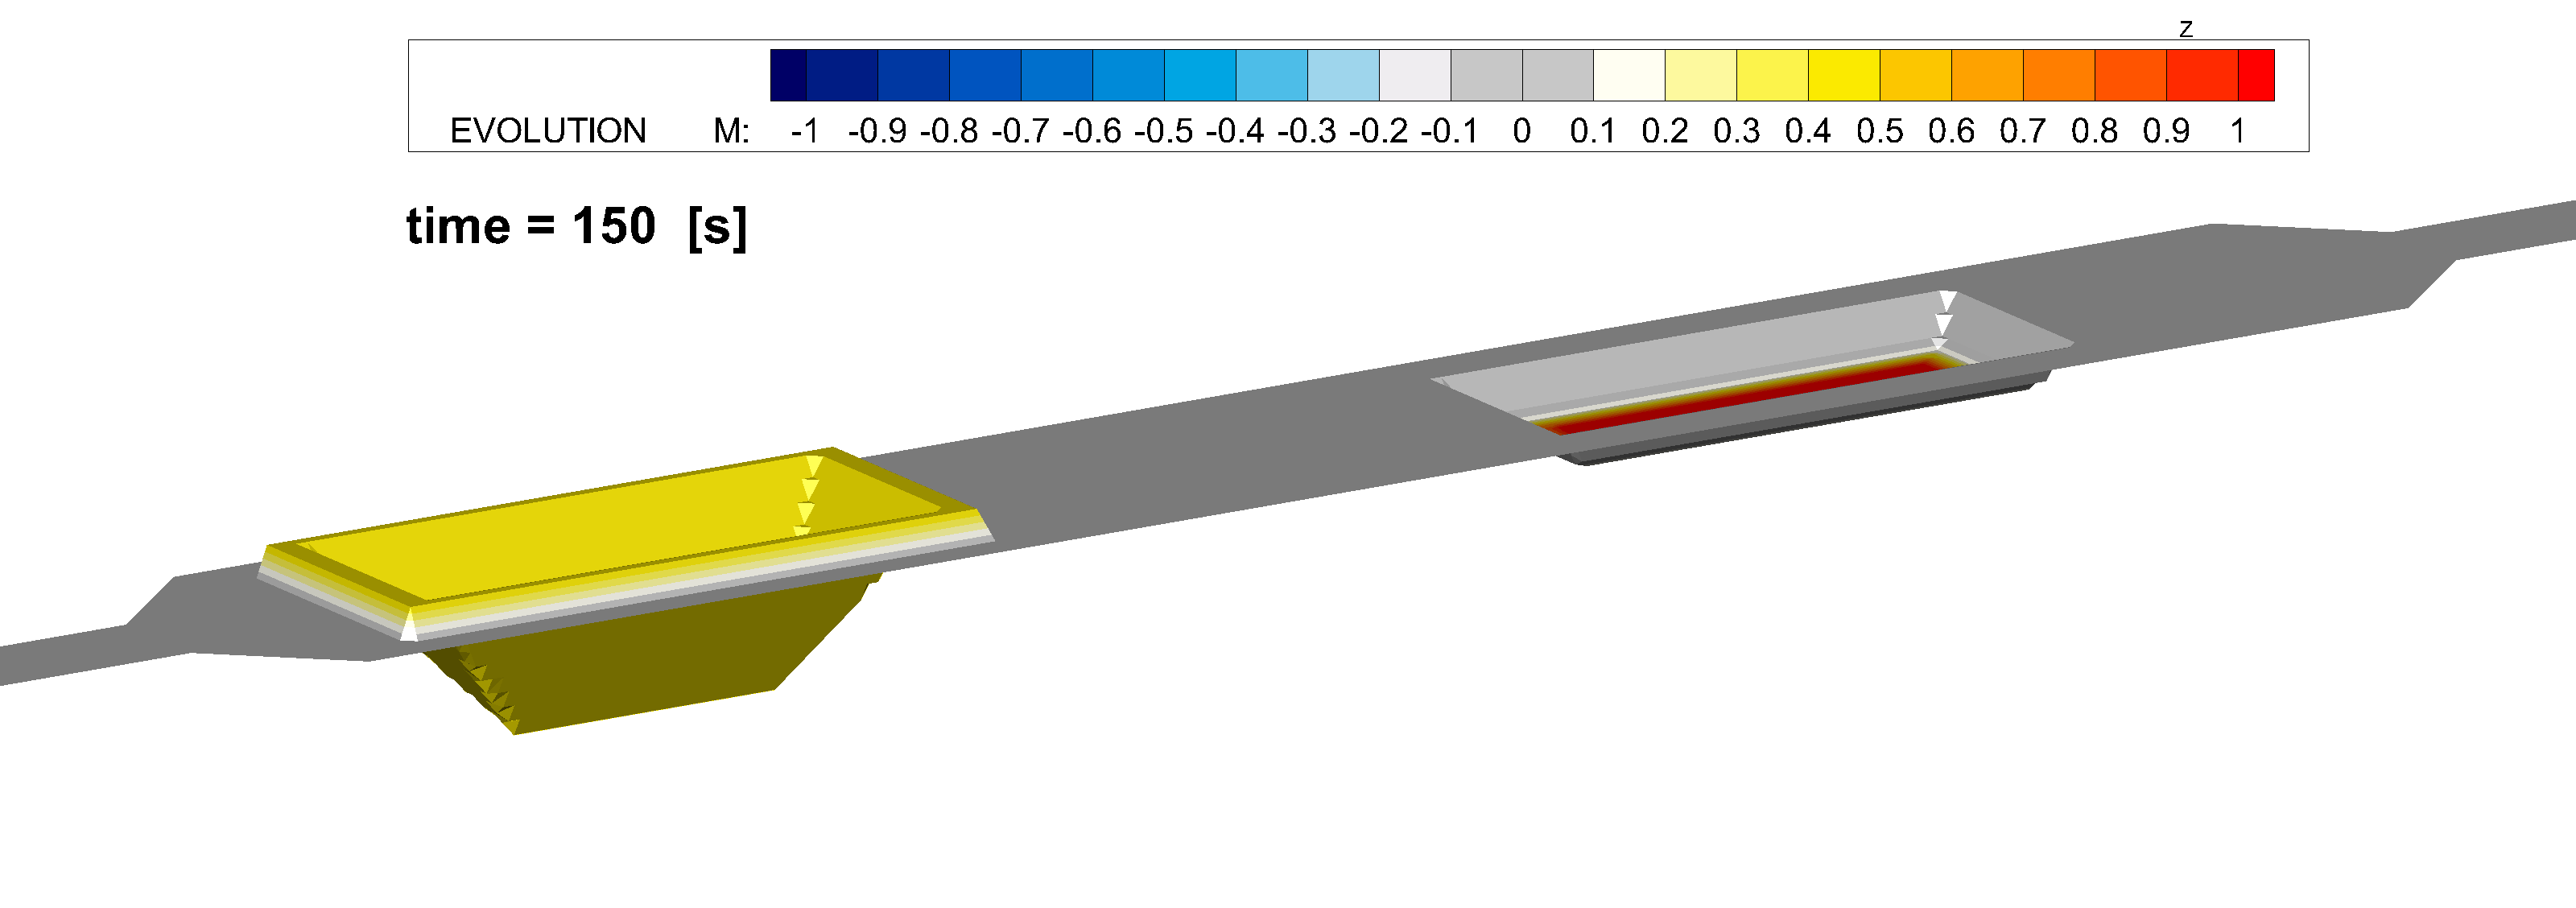
\includegraphics[scale=0.14]{../img/result150_zoom3D.png}
%\caption{Simulated evolution after 0s and 150 s.}\label{result3D}
%\end{figure}


